\documentclass[11pt,a4paper]{article}
\usepackage{fontspec}
\setmainfont{DejaVu Serif}[Scale=0.92]
\setsansfont{DejaVu Sans}[Scale=0.92]
\setmonofont{DejaVu Sans Mono}[Scale=0.82]
\usepackage[margin=2.2cm]{geometry}
\usepackage{microtype}
\usepackage{xcolor}
\usepackage{tikz}
\usetikzlibrary{arrows.meta,positioning,shapes.geometric,shapes.multipart,fit,backgrounds,calc,decorations.pathreplacing}
\usepackage{booktabs,tabularx,array,longtable,needspace}
\usepackage{enumitem}
\usepackage{caption}
\usepackage{float}
\usepackage{fancyvrb}
\usepackage[colorlinks=true,linkcolor=blue!50!black,urlcolor=blue!50!black]{hyperref}

\definecolor{sw}{HTML}{DCEBFA}      % switch
\definecolor{swd}{HTML}{2B6CB0}
\definecolor{ct}{HTML}{E6F4EA}      % controller
\definecolor{ctd}{HTML}{2F855A}
\definecolor{ho}{HTML}{FFF4E0}      % hosts
\definecolor{hod}{HTML}{B7791F}
\definecolor{rf}{HTML}{F3E8FD}      % reference / test
\definecolor{rfd}{HTML}{6B46C1}
\definecolor{bad}{HTML}{C53030}

\tikzset{
  box/.style={draw, rounded corners=2pt, align=center, minimum height=9mm, inner sep=4pt, font=\small},
  swbox/.style={box, fill=sw, draw=swd},
  ctbox/.style={box, fill=ct, draw=ctd},
  hobox/.style={box, fill=ho, draw=hod},
  rfbox/.style={box, fill=rf, draw=rfd},
  dec/.style={draw, diamond, aspect=2.2, align=center, inner sep=1pt, font=\small, fill=white},
  term/.style={draw, rounded corners=8pt, align=center, font=\small, inner sep=4pt, fill=gray!8},
  arr/.style={-{Stealth[length=2.2mm]}, thick},
  lbl/.style={font=\scriptsize, fill=white, inner sep=1pt},
  st/.style={draw, circle, align=center, font=\scriptsize, minimum size=15mm, inner sep=1pt},
}

\newcommand{\code}[1]{\texttt{#1}}
\setlist{nosep, leftmargin=*}
\setlength{\parindent}{0pt}
\setlength{\parskip}{5pt}

\title{\textbf{ja4p4}\\[2pt]\large JA4+ fingerprinting in a P4 switch: design, decisions and how each problem is solved}
\author{Working document, updated as the code is written}
\date{Version of \today}

\begin{document}
\maketitle
\tableofcontents
\newpage

%=====================================================================
\section{What the project does}

Before most network protocols begin their real, often encrypted, conversation, the two sides exchange a few
messages in the clear: the TCP handshake, the TLS ClientHello and ServerHello, the SSH banner, a plain HTTP request,
a DHCP request. How a program builds these messages depends on its operating system, library and configuration, so
the messages identify the software that sent them. The JA4+ suite (by FoxIO) turns each of them into a short,
stable text fingerprint.

This project computes the JA4+ fingerprints of the traffic that passes through a P4 switch, and requires each value
to equal the one FoxIO's own tool computes from the same packets. The contribution is that the fingerprinting is
done in the switch's P4 pipeline. Nothing else is in scope: no flood protection, no hardware port, no performance
tuning.

\textbf{What is done and what is not} is summarised, with the reason for each gap, in
Section~\ref{sec:coverage}.

\textbf{Status of this document.} It grows with the code. Every number in it comes from a run of the code at the version it describes.

%=====================================================================
\section{Setup}

\begin{figure}[H]\centering
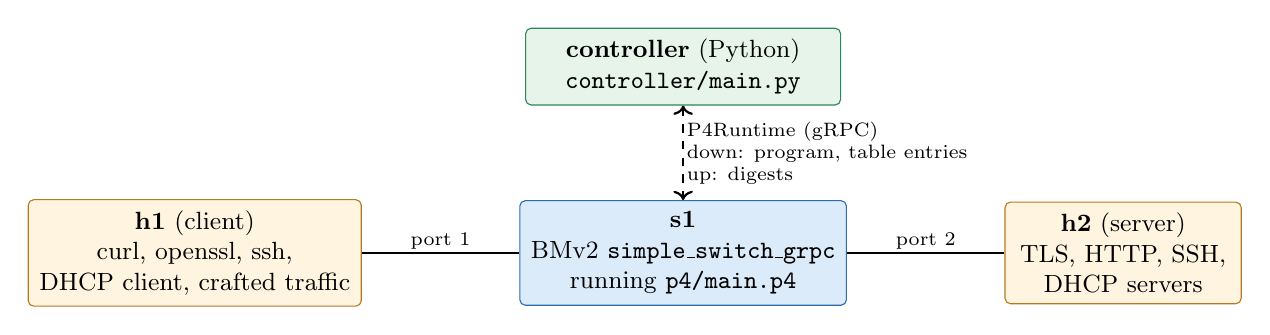
\begin{tikzpicture}[node distance=14mm and 20mm]
  \node[hobox, minimum width=30mm] (h1) {\textbf{h1} (client)\\ curl, openssl, ssh,\\ DHCP client, crafted traffic};
  \node[swbox, minimum width=34mm, right=of h1] (s1) {\textbf{s1}\\ BMv2 \code{simple\_switch\_grpc}\\ running \code{p4/main.p4}};
  \node[hobox, minimum width=30mm, right=of s1] (h2) {\textbf{h2} (server)\\ TLS, HTTP, SSH,\\ DHCP servers};
  \node[ctbox, minimum width=40mm, above=12mm of s1] (c) {\textbf{controller} (Python)\\ \code{controller/main.py}};
  \draw[thick] (h1) -- node[lbl, above]{port 1} (s1);
  \draw[thick] (s1) -- node[lbl, above]{port 2} (h2);
  \draw[arr, <->, dashed] (c) -- node[lbl, right, align=left]{P4Runtime (gRPC)\\ down: program, table entries\\ up: digests} (s1);
\end{tikzpicture}
\caption{The network: one switch, two hosts, one controller.}
\end{figure}

\begin{itemize}
\item \textbf{Live runs} use Mininet: h1 and h2 are network namespaces joined to the switch's ports 1 and 2.
\item \textbf{Tests} run the same switch binary and the same compiled program without root: the switch takes its
  packets through a nanomsg socket instead of network interfaces, and a test program sends captured frames into
  it (Section~\ref{sec:testing}).
\end{itemize}

%=====================================================================
\section{Architecture}

\subsection{Who does what}

The rule: \emph{the switch does everything P4 can do per packet}: parse, read every field a fingerprint uses, keep
small per-connection state, count, compute arithmetic such as latencies. \emph{The controller does what P4 cannot}:
write text, sort variable-length lists, compute SHA-256 and a histogram's mode, and hold the bytes of a message
that is spread over several packets until it is complete. The controller never reads a field of a message: when it
has joined the pieces, it sends the joined message back into the switch, which reads it with the same parser.

\begin{figure}[H]\centering
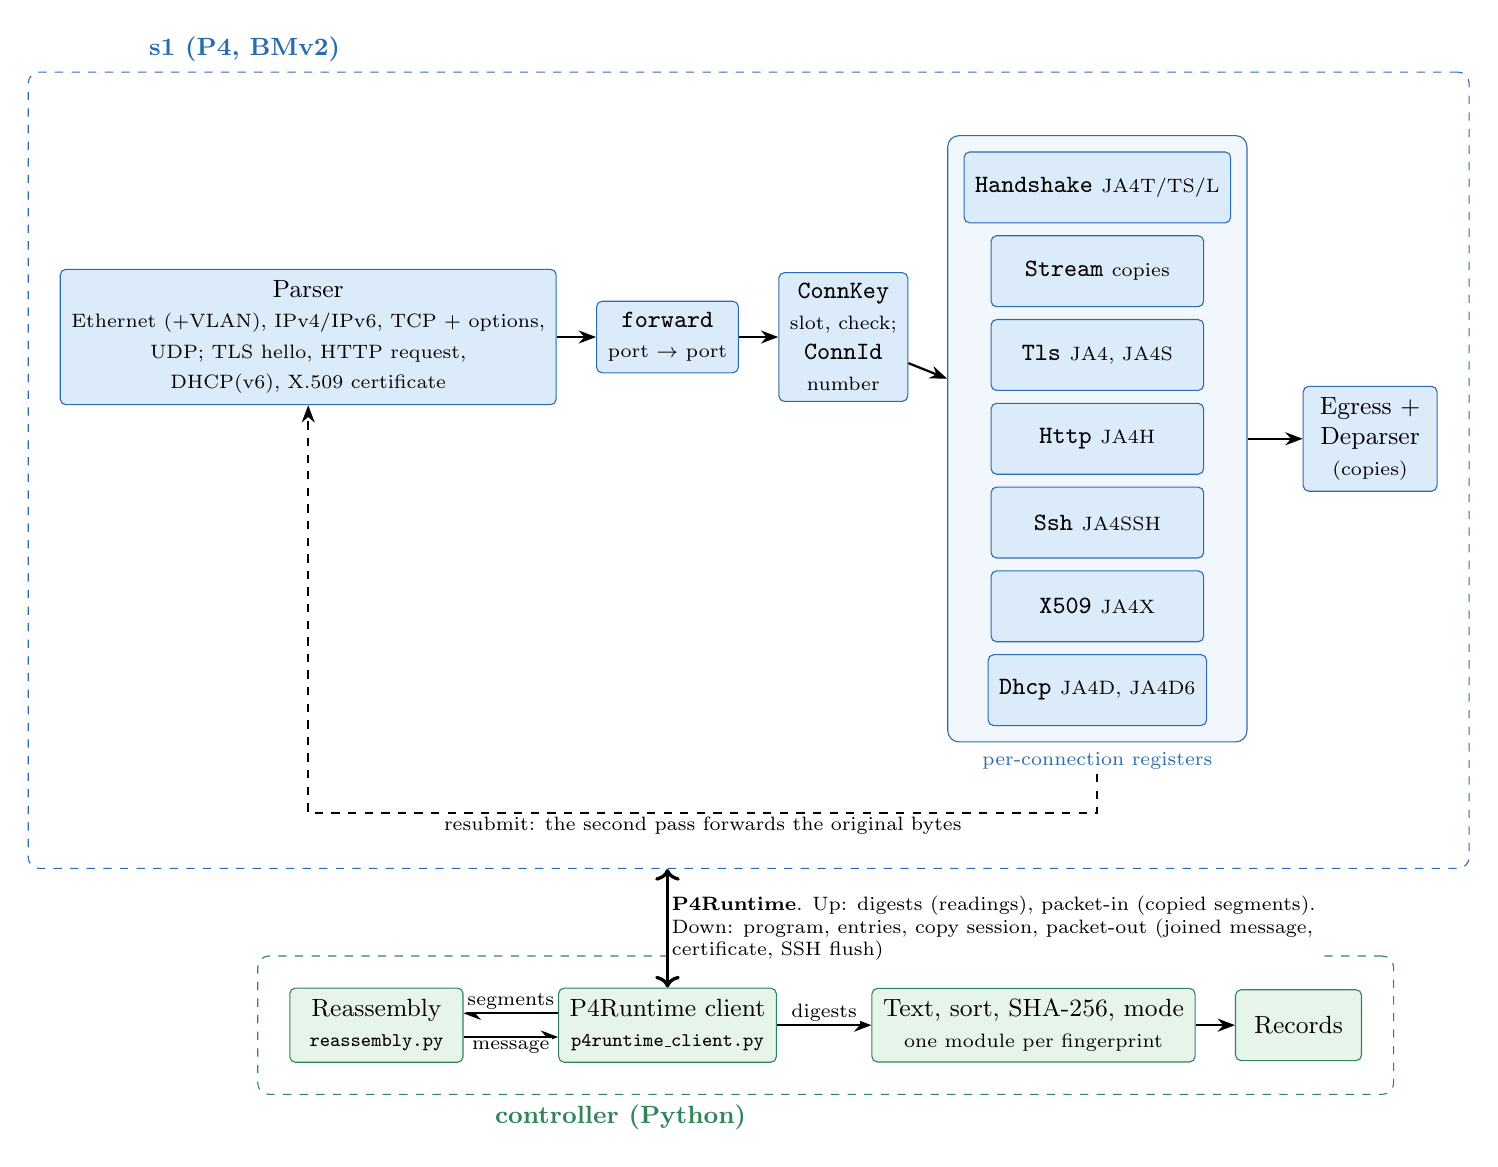
\begin{tikzpicture}[node distance=5mm]
  \node[swbox, minimum width=27mm] (prs) {Parser\\ \scriptsize Ethernet (+VLAN), IPv4/IPv6, TCP + options,\\ \scriptsize UDP; TLS hello, HTTP request,\\ \scriptsize DHCP(v6), X.509 certificate};
  \node[swbox, minimum width=18mm, right=5mm of prs] (fwd) {\code{forward}\\ \scriptsize port $\rightarrow$ port};
  \node[swbox, minimum width=16mm, right=5mm of fwd] (ck) {\code{ConnKey}\\ \scriptsize slot, check;\\ \code{ConnId}\\ \scriptsize number};
  \node[swbox, minimum width=27mm, right=7mm of ck, yshift=19mm] (hs) {\code{Handshake} \scriptsize JA4T/TS/L};
  \node[swbox, minimum width=27mm, below=1.5mm of hs] (st) {\code{Stream} \scriptsize copies};
  \node[swbox, minimum width=27mm, below=1.5mm of st] (tl) {\code{Tls} \scriptsize JA4, JA4S};
  \node[swbox, minimum width=27mm, below=1.5mm of tl] (ht) {\code{Http} \scriptsize JA4H};
  \node[swbox, minimum width=27mm, below=1.5mm of ht] (sh) {\code{Ssh} \scriptsize JA4SSH};
  \node[swbox, minimum width=27mm, below=1.5mm of sh] (x5) {\code{X509} \scriptsize JA4X};
  \node[swbox, minimum width=27mm, below=1.5mm of x5] (dh) {\code{Dhcp} \scriptsize JA4D, JA4D6};
  \begin{scope}[on background layer]
    \node[draw=swd, fill=sw!40, rounded corners, fit=(hs)(dh), inner sep=2mm, label={[font=\scriptsize, text=swd, align=center]below:per-connection registers}] (regs) {};
  \end{scope}
  \node[swbox, minimum width=17mm, right=7mm of regs] (eg) {Egress +\\ Deparser\\ \scriptsize (copies)};
  \draw[arr] (prs) -- (fwd); \draw[arr] (fwd) -- (ck); \draw[arr] (ck) -- (regs); \draw[arr] (regs) -- (eg);
  \draw[arr, dashed] (regs.south) ++(0,-4mm) -- ++(0,-5mm) -| node[lbl, pos=0.25, below]{resubmit: the second pass forwards the original bytes} (prs.south);
  \begin{scope}[on background layer]
    \node[draw=swd, dashed, rounded corners, fit=(prs)(eg)(regs), inner xsep=4mm, inner ysep=12mm, yshift=-4mm, label={[font=\small\bfseries, text=swd]above left:s1 (P4, BMv2)}] (swf) {};
  \end{scope}
  \node[ctbox, below=78mm of fwd, minimum width=26mm] (p4rt) {P4Runtime client\\ \scriptsize \code{p4runtime\_client.py}};
  \node[ctbox, left=12mm of p4rt, minimum width=22mm] (ras) {Reassembly\\ \scriptsize \code{reassembly.py}};
  \node[ctbox, right=12mm of p4rt, minimum width=36mm] (fmt) {Text, sort, SHA-256, mode\\ \scriptsize one module per fingerprint};
  \node[ctbox, right=5mm of fmt, minimum width=16mm] (rec) {Records};
  \begin{scope}[on background layer]
    \node[draw=ctd, dashed, rounded corners, fit=(ras)(rec), inner sep=4mm, label={[font=\small\bfseries, text=ctd]below left:controller (Python)}] {};
  \end{scope}
  \draw[arr, <->, very thick] (p4rt.north) -- node[lbl, right, align=left, pos=0.5]{\textbf{P4Runtime}. Up: digests (readings), packet-in (copied segments).\\ Down: program, entries, copy session, packet-out (joined message,\\ certificate, SSH flush)} (p4rt.north |- swf.south);
  \draw[arr] ($(p4rt.west)+(0,1.5mm)$) -- node[lbl, above]{segments} ($(ras.east)+(0,1.5mm)$);
  \draw[arr] ($(ras.east)+(0,-1.5mm)$) -- node[lbl, below]{message} ($(p4rt.west)+(0,-1.5mm)$);
  \draw[arr] (p4rt) -- node[lbl, above]{digests} (fmt); \draw[arr] (fmt) -- (rec);
\end{tikzpicture}
\caption{Components. Blue: the P4 program in the switch. Green: the controller. Every channel between them is
P4Runtime.}
\end{figure}

\subsection{Files}

\begin{tabularx}{\textwidth}{>{\ttfamily}l X}
\toprule
p4/main.p4 & top level: \code{ConnKey}, \code{ConnId} (the connection's number), forwarding, which controls run for which packet, egress (copies), deparser \\
p4/headers.p4 & headers (including packet-in / packet-out) and metadata \\
p4/parser.p4 & parser: Ethernet and up to two VLAN tags, IP, TCP and the TCP option walk, UDP; first and second pass; packet-out \\
p4/parser\_tls.p4, parser\_http.p4, parser\_dhcp.p4, parser\_x509.p4 & the message walks (included in the parser) \\
p4/handshake.p4 & JA4T, JA4TS, JA4L \\
p4/stream.p4 & per-direction stream state: which segments are copied to the controller \\
p4/tls.p4, http.p4, ssh.p4, dhcp.p4, x509.p4 & one control per fingerprint family: counts, state, the digest \\
controller/main.py & connects, loads the program, installs forwarding and the copy session, handles digests and packet-in, finishes (SSH flush) \\
controller/p4runtime\_client.py & minimal P4Runtime client (arbitration, pipeline, entries, clone session, digests, packet-in/out) \\
controller/handshake.py, tls.py, http.py, ssh.py, dhcp.py, x509.py & the text of each fingerprint from its digest \\
controller/reassembly.py & joins the copied segments of a split message; cuts certificates out of a server flight \\
controller/records.py & one record per connection (endpoints and the switch's connection number) \\
tools/live\_tex.py & the live run's results table for both PDFs \\
tools/replay.py & runs switch + controller without root and replays a capture \\
tools/reference.py, compare.py & reference fingerprints (FoxIO's tool, tshark, FoxIO's Wireshark plugin output) and the verdict per fingerprint; forwarding check \\
tests/ & 11 files, 27 tests (Section~\ref{sec:testing} and the tested cases of the split section) \\
\bottomrule
\end{tabularx}

\subsection{Life of a packet}

\begin{figure}[H]\centering
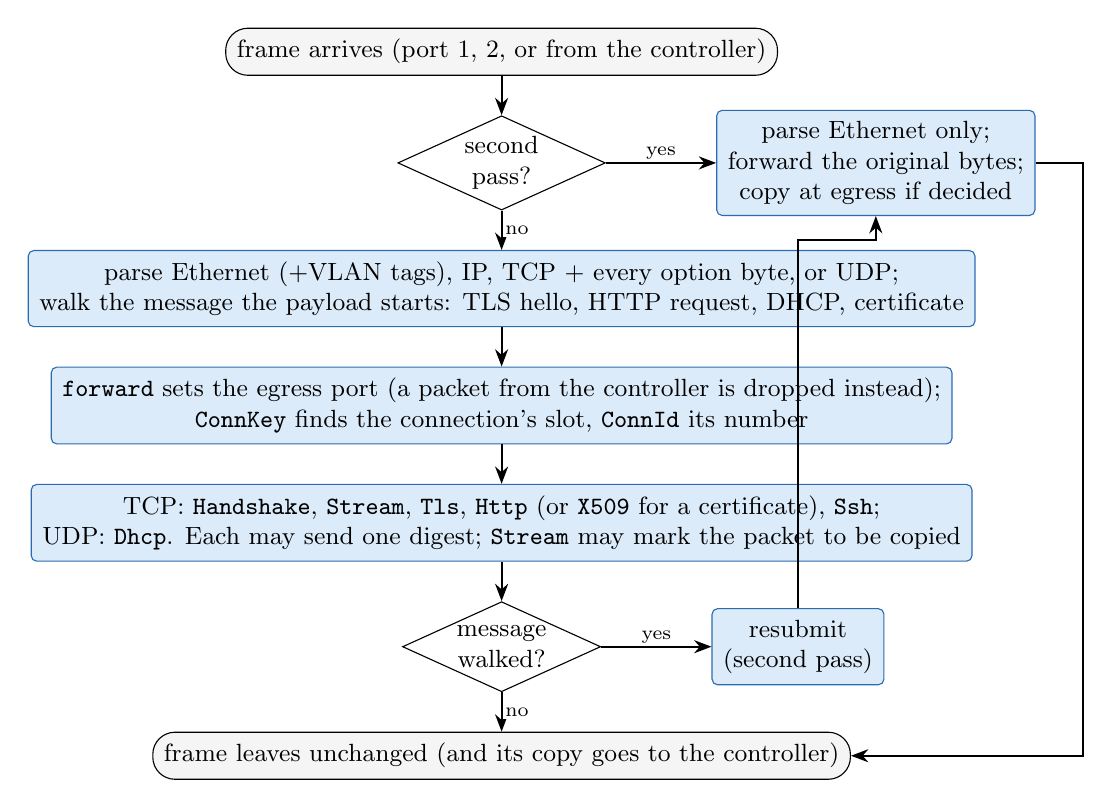
\begin{tikzpicture}[node distance=5mm]
  \node[term] (in) {frame arrives (port 1, 2, or from the controller)};
  \node[dec, below=of in] (rs) {second\\ pass?};
  \node[swbox, right=14mm of rs] (p2) {parse Ethernet only;\\ forward the original bytes;\\ copy at egress if decided};
  \node[swbox, below=of rs, minimum width=80mm] (p) {parse Ethernet (+VLAN tags), IP, TCP + every option byte, or UDP;\\ walk the message the payload starts: TLS hello, HTTP request, DHCP, certificate};
  \node[swbox, below=of p, minimum width=80mm] (f) {\code{forward} sets the egress port (a packet from the controller is dropped instead);\\ \code{ConnKey} finds the connection's slot, \code{ConnId} its number};
  \node[swbox, below=of f, minimum width=80mm] (h) {TCP: \code{Handshake}, \code{Stream}, \code{Tls}, \code{Http} (or \code{X509} for a certificate), \code{Ssh};\\ UDP: \code{Dhcp}. Each may send one digest; \code{Stream} may mark the packet to be copied};
  \node[dec, below=of h] (w) {message\\ walked?};
  \node[swbox, right=14mm of w] (re) {resubmit\\ (second pass)};
  \node[term, below=of w] (out) {frame leaves unchanged (and its copy goes to the controller)};
  \draw[arr] (in) -- (rs);
  \draw[arr] (rs) -- node[lbl, above]{yes} (p2);
  \draw[arr] (rs) -- node[lbl, right]{no} (p);
  \draw[arr] (p) -- (f); \draw[arr] (f) -- (h); \draw[arr] (h) -- (w);
  \draw[arr] (w) -- node[lbl, above]{yes} (re);
  \draw[arr] (w) -- node[lbl, right]{no} (out);
  \draw[arr] (re.north) |- ($(p2.south)+(0,-3mm)$) -- (p2.south);
  \draw[arr] (p2.east) -- ++(6mm,0) |- (out.east);
\end{tikzpicture}
\caption{What the switch does with every frame. Fingerprinting only reads the packet; every frame leaves exactly as
it arrived (checked for every frame of every test). Only frames whose payload the parser walked take a second
pass.}
\end{figure}

%=====================================================================
\section{TCP handshake fingerprints: JA4T, JA4TS, JA4L}

\subsection{What is measured}

\begin{figure}[H]\centering
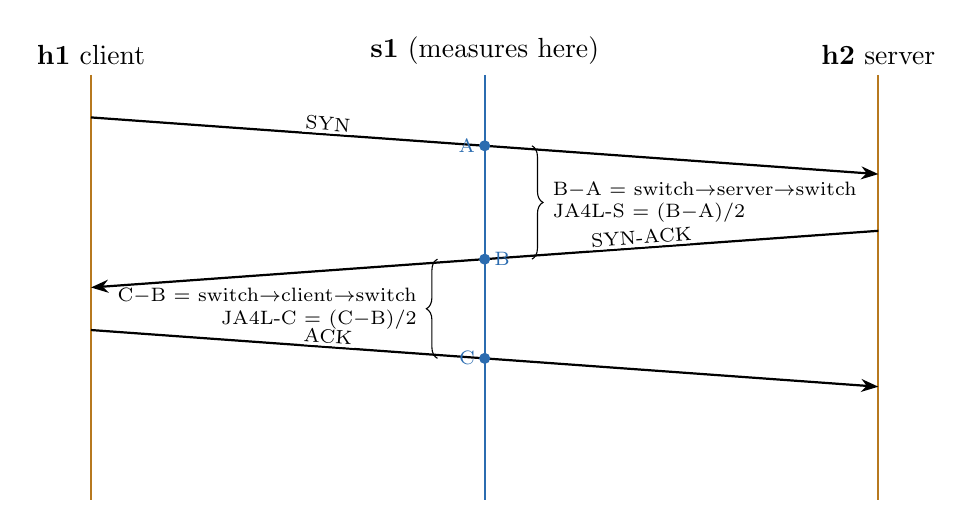
\begin{tikzpicture}[x=1cm,y=-0.9cm]
  \draw[thick, hod] (0,0) node[above, black]{\textbf{h1} client} -- (0,6);
  \draw[thick, swd] (5,0) node[above, black]{\textbf{s1} (measures here)} -- (5,6);
  \draw[thick, hod] (10,0) node[above, black]{\textbf{h2} server} -- (10,6);
  \draw[arr] (0,0.6) -- (10,1.4) node[pos=0.3, lbl, above, sloped]{SYN};
  \fill[swd] (5,1.0) circle (2pt) node[left, font=\scriptsize]{A};
  \draw[arr] (10,2.2) -- (0,3.0) node[pos=0.3, lbl, above, sloped]{SYN-ACK};
  \fill[swd] (5,2.6) circle (2pt) node[right, font=\scriptsize]{B};
  \draw[arr] (0,3.6) -- (10,4.4) node[pos=0.3, lbl, above, sloped]{ACK};
  \fill[swd] (5,4.0) circle (2pt) node[left, font=\scriptsize]{C};
  \draw[decorate, decoration={brace, amplitude=4pt}] (5.6,1.0) -- (5.6,2.6) node[midway, right=4pt, font=\scriptsize, align=left]{B$-$A = switch$\to$server$\to$switch\\ JA4L-S = (B$-$A)/2};
  \draw[decorate, decoration={brace, amplitude=4pt, mirror}] (4.4,2.6) -- (4.4,4.0) node[midway, left=4pt, font=\scriptsize, align=right]{C$-$B = switch$\to$client$\to$switch\\ JA4L-C = (C$-$B)/2};
\end{tikzpicture}
\caption{JA4L: the switch timestamps the three handshake packets. Each half is a one-way latency estimate from the
switch to one side.}
\end{figure}

\begin{tabularx}{\textwidth}{l X l}
\toprule
\textbf{Fingerprint} & \textbf{Format (FoxIO)} & \textbf{Example} \\
\midrule
JA4T & window \_ option kinds in order, joined by - \_ MSS \_ window scale (from the client SYN) & \code{64240\_2-1-3-1-1-4\_1460\_8} \\
JA4TS & the same, from the server SYN-ACK & \code{65535\_2-1-3-1-1-4\_1460\_8} \\
JA4L-C & (C$-$B)/2 in µs \_ client TTL & \code{62\_128} \\
JA4L-S & (B$-$A)/2 in µs \_ server TTL & \code{33804\_227} \\
\bottomrule
\end{tabularx}

Details copied from FoxIO's Rust code (\code{tcp.rs}, \code{time/tcp.rs}): no options gives \code{00}; a missing MSS
gives \code{00}; window scale 0 or missing gives \code{00}, otherwise the plain number; the TTL is the raw value seen,
not a hop count; latencies are integer microseconds, halved with truncation.

\subsection{Parsing the TCP options in P4}

\textbf{Problem.} The options are a variable list (0--40 bytes) of variable-length items. JA4T needs the kind of
every item in order, plus the MSS and window-scale values.

\textbf{Approach: walk the options one byte at a time.} Each byte is extracted into a stack of one-byte headers
(\code{hdr.tcp\_opt}, 40 entries), and a small state machine reads them. A counter \code{left} starts at
$4\cdot$\code{dataOffset}$-20$ and decreases with every byte, so the walk can never run into the payload.

\textbf{Why this approach.}
\begin{itemize}
\item \emph{Every byte is kept.} Bytes the parser skips are dropped from the packet in BMv2 (\code{advance}
  discards them). Extracting each byte into a header lets the deparser emit the options unchanged, so forwarding is
  not affected by fingerprinting.
\item \emph{Any order and any option.} No assumption about which options a SYN carries; unknown kinds are skipped by
  their length byte.
\item \emph{Bounded.} At most 40 iterations; the list of kinds fits in a 320-bit field (40 bytes), so even a SYN made
  of 40 NOPs is recorded completely: there is no truncation case.
\end{itemize}

\begin{figure}[H]\centering
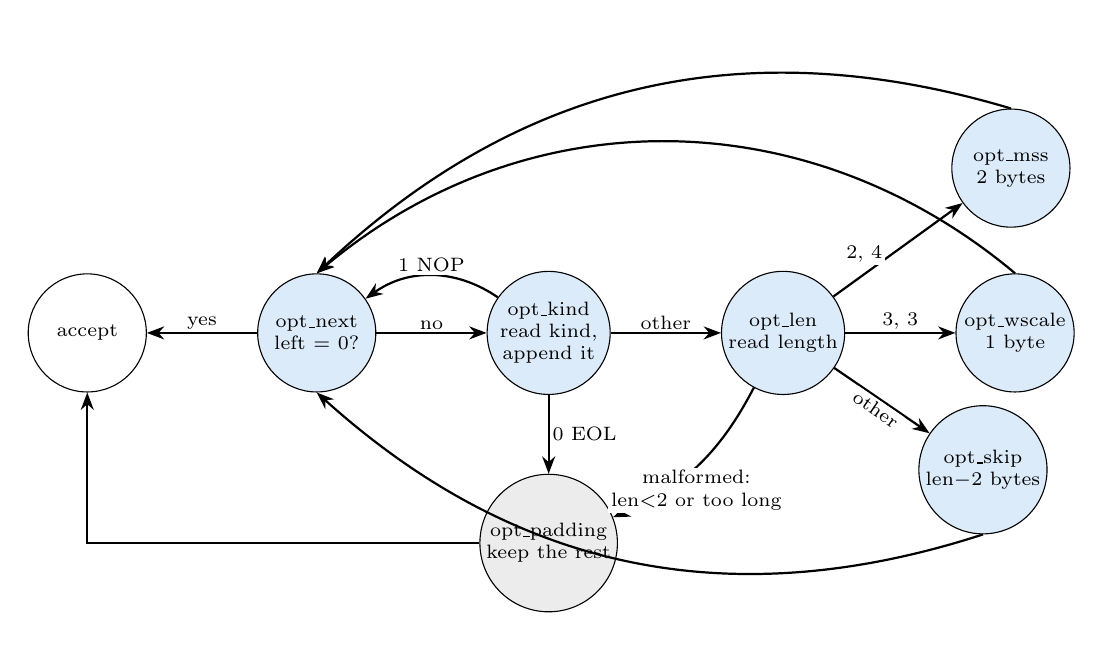
\begin{tikzpicture}[node distance=10mm and 14mm, every node/.style={font=\scriptsize}]
  \node[st, fill=sw] (next) {opt\_next\\ left = 0?};
  \node[st, fill=sw, right=of next] (kind) {opt\_kind\\ read kind,\\ append it};
  \node[st, fill=sw, right=of kind] (len) {opt\_len\\ read length};
  \node[st, fill=sw, above right=10mm and 18mm of len] (mss) {opt\_mss\\ 2 bytes};
  \node[st, fill=sw, right=of len] (ws) {opt\_wscale\\ 1 byte};
  \node[st, fill=sw, below right=6mm and 14mm of len] (skip) {opt\_skip\\ len$-$2 bytes};
  \node[st, fill=gray!15, below=of kind] (pad) {opt\_padding\\ keep the rest};
  \node[st, fill=white, left=of next] (acc) {accept};
  \draw[arr] (next) -- node[lbl, above]{no} (kind);
  \draw[arr] (next) -- node[lbl, above]{yes} (acc);
  \draw[arr] (kind) to[bend right=35] node[lbl, above]{1 NOP} (next);
  \draw[arr] (kind) -- node[lbl, right]{0 EOL} (pad);
  \draw[arr] (kind) -- node[lbl, above]{other} (len);
  \draw[arr] (len) -- node[lbl, pos=0.45, left=2pt]{2, 4} (mss);
  \draw[arr] (len) -- node[lbl, above]{3, 3} (ws);
  \draw[arr] (len) -- node[lbl, sloped, below]{other} (skip);
  \draw[arr] (len) to[bend left=20] node[lbl, below, align=center]{malformed:\\ len$<$2 or too long} (pad);
  \draw[arr] (mss.north) to[bend right=30] (next.north);
  \draw[arr] (ws.north) to[bend right=40] (next.north);
  \draw[arr] (skip.south) to[bend left=30] (next.south);
  \draw[arr] (pad) -| (acc);
\end{tikzpicture}
\caption{The TCP option walk (\code{p4/parser.p4}). Every arrow extracts one or more bytes and decreases \code{left}.}
\end{figure}

\textbf{A bug found and its fix.} The first version read each byte back through \code{hdr.tcp\_opt.last} after
extracting it. MSS 1460 (bytes \code{05 B4}) came out as 46260 (\code{B4 B4}): both reads returned the second byte,
even after splitting them into two parser states. The parser now reads each value with \code{lookahead} \emph{before}
extracting the byte, which does not depend on how the compiler resolves \code{.last}. After the change the MSS
values equal FoxIO's.

\subsection{Per-connection state for JA4L}

\textbf{Problem.} JA4L needs times from three different packets, two of them travelling in the opposite direction
to the third. Something must remember A and B until C arrives.

\textbf{Approach: the switch keeps the state and does the arithmetic.} A register array of 65,536 slots holds, per
connection: a check value, a state, time A, time B, client TTL, server TTL. When C passes, the switch computes both
halves and sends finished numbers. The controller only writes them as text.

\textbf{Finding a connection's slot from either direction} (control \code{ConnKey} in \code{main.p4}, shared by
every fingerprint that keeps state). The endpoints are put in a fixed order (the smaller
(address, port) pair first), so a client$\to$server packet and a server$\to$client packet produce the same key:
\begin{center}
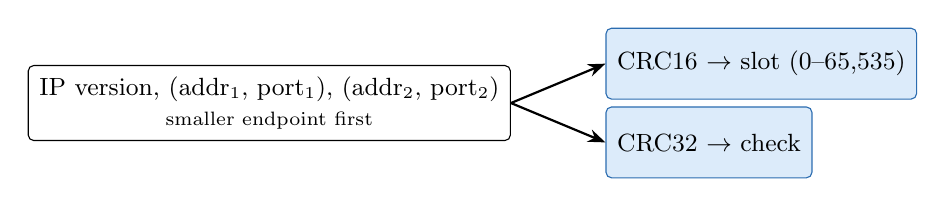
\begin{tikzpicture}[node distance=6mm]
  \node[box] (k) {IP version, (addr$_1$, port$_1$), (addr$_2$, port$_2$)\\ \scriptsize smaller endpoint first};
  \node[swbox, right=12mm of k, yshift=5mm] (s) {CRC16 $\rightarrow$ slot (0--65,535)};
  \node[swbox, right=12mm of k, yshift=-5mm] (c) {CRC32 $\rightarrow$ check};
  \draw[arr] (k.east) -- (s.west); \draw[arr] (k.east) -- (c.west);
\end{tikzpicture}
\end{center}
A slot belongs to a connection only if its stored check equals the connection's check. Two connections that share a
slot are told apart by the check; the newer SYN takes the slot (a simple, documented rule).

\textbf{The connection's number} (control \code{ConnId} in \code{main.p4}). The endpoints alone do not identify a
connection: a client, or a NAT, reuses addresses and ports for a new connection after the old one closed. ConnId
gives each connection a number from a counter: a new one when another connection (a different check) comes to the
slot, and when a SYN with a new initial sequence number arrives on the same endpoints; a repeated SYN keeps the
number. Every control keeps its per-connection state with this number (it replaced the check in each control), and
every TCP digest and every copy for the controller carries it, so the controller keeps one record per connection.
Before this, the second connection on reused ports lost its JA4 and two SSH sessions were counted into one wrong
JA4SSH (\code{tests/test\_port\_reuse.py}, red then green). On the SYN of a reused port, the previous SSH
connection's last window is reported; the SYN's own handshake digest then goes out on a second pass (one digest per
packet on BMv2).

\begin{figure}[H]\centering
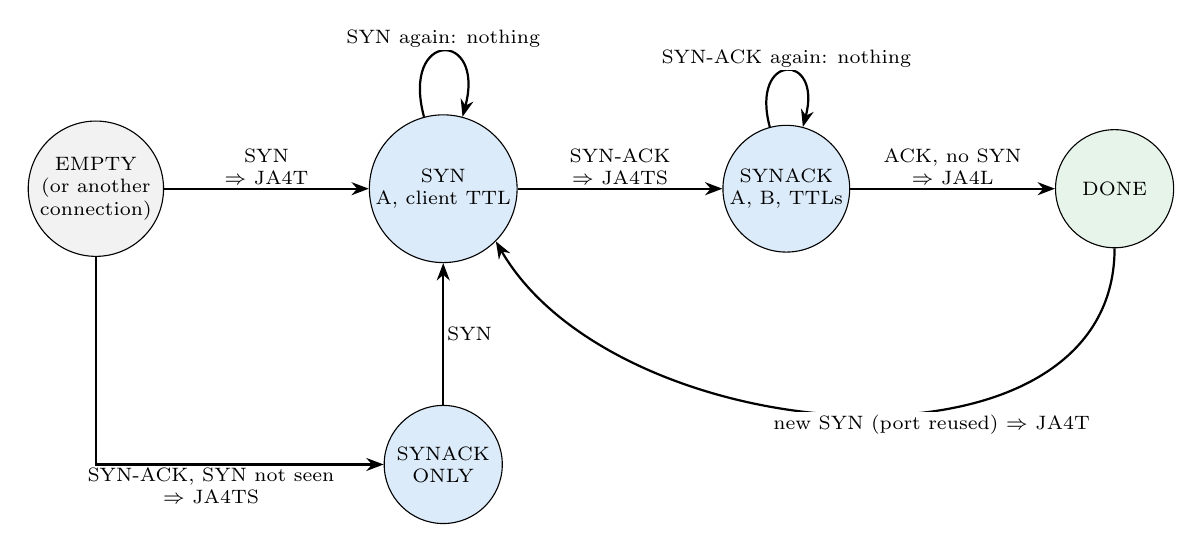
\begin{tikzpicture}[node distance=12mm and 26mm, every node/.style={font=\scriptsize}]
  \node[st, fill=gray!10] (e) {EMPTY\\ (or another\\ connection)};
  \node[st, fill=sw, right=of e] (s) {SYN\\ A, client TTL};
  \node[st, fill=sw, right=of s] (sa) {SYNACK\\ A, B, TTLs};
  \node[st, fill=ct, right=of sa] (d) {DONE};
  \node[st, fill=sw, below=18mm of s] (so) {SYNACK\\ ONLY};
  \draw[arr] (e) -- node[lbl, above, align=center]{SYN\\ $\Rightarrow$ JA4T} (s);
  \draw[arr] (s) -- node[lbl, above, align=center]{SYN-ACK\\ $\Rightarrow$ JA4TS} (sa);
  \draw[arr] (sa) -- node[lbl, above, align=center]{ACK, no SYN\\ $\Rightarrow$ JA4L} (d);
  \draw[arr] (e) |- node[lbl, pos=0.7, below, align=center]{SYN-ACK, SYN not seen\\ $\Rightarrow$ JA4TS} (so);
  \draw[arr] (d.south) to[out=-90,in=-60] node[lbl, below, pos=0.4]{new SYN (port reused) $\Rightarrow$ JA4T} (s.south east);
  \draw[arr] (so) -- node[lbl, right]{SYN} (s);
  \draw[arr] (s) to[loop above, looseness=6] node[lbl, above]{SYN again: nothing} (s);
  \draw[arr] (sa) to[loop above, looseness=6] node[lbl, above]{SYN-ACK again: nothing} (sa);
\end{tikzpicture}
\caption{The per-connection state in \code{p4/handshake.p4}. The order follows FoxIO's reference: the first SYN,
then the first SYN-ACK, then the first packet with ACK and without SYN, from either side. Retransmissions change
nothing.}
\label{fig:hsflow}
\end{figure}

\textbf{Why in the switch, not the controller.} Sending every handshake packet's time to the controller would work,
but it would move the measurement out of the data plane, and the times would be those of packets delivered to
software. Keeping A and B in registers costs six register reads and writes per handshake packet and sends one
message per fingerprint, not per packet.

\subsection{From switch to controller: the digest}

All three fingerprints share one digest type, \code{hs\_digest\_t}: a \code{kind} (1 JA4T, 2 JA4TS, 3 JA4L), the
packet's endpoints, the TCP fields (window, option count, the 320-bit list of kinds, MSS, window scale, which of the
two were present), and the JA4L values (two latencies, two TTLs).

\textbf{A bug found and its fix: one digest call, not four.} The first version called \code{digest()} in each of
four branches. The controller received JA4L for a connection about a second \emph{before} its JA4T. The cause: the
compiler creates one BMv2 learn list per call site, all named \code{hs\_digest\_t}; the controller's digest
configuration (send at once) reached only one of them, and the other three used BMv2's default batching. The
control now fills the digest in its branches and calls \code{digest()} once at the end; the compiled program has a
single learn list and every fingerprint arrives in packet order.

%=====================================================================
\section{TLS fingerprints: JA4 and JA4S}

\subsection{What is read}

\begin{figure}[H]\centering
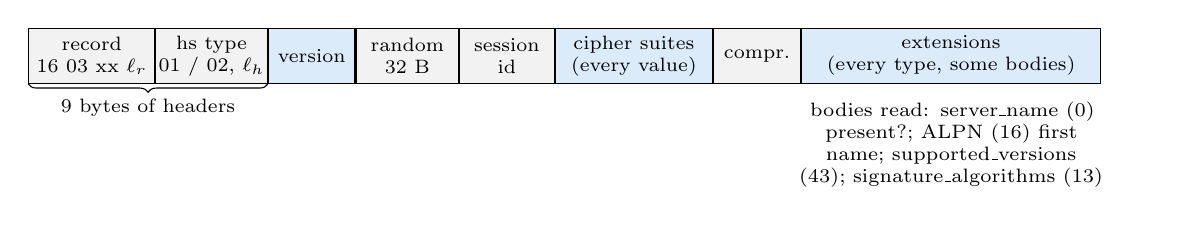
\begin{tikzpicture}[x=1mm, y=1mm, every node/.style={font=\scriptsize}]
  \tikzset{fld/.style={draw, minimum height=7mm, inner sep=1pt, align=center}}
  \node[fld, fill=gray!10, minimum width=16mm, anchor=west] (r) at (0,0) {record\\ 16 03 xx $\ell_r$};
  \node[fld, fill=gray!10, minimum width=14mm, right=0mm of r] (h) {hs type\\ 01 / 02, $\ell_h$};
  \node[fld, fill=sw, minimum width=11mm, right=0mm of h] (v) {version};
  \node[fld, fill=gray!10, minimum width=13mm, right=0mm of v] (rnd) {random\\ 32 B};
  \node[fld, fill=gray!10, minimum width=12mm, right=0mm of rnd] (sid) {session\\ id};
  \node[fld, fill=sw, minimum width=20mm, right=0mm of sid] (cs) {cipher suites\\ (every value)};
  \node[fld, fill=gray!10, minimum width=11mm, right=0mm of cs] (cm) {compr.};
  \node[fld, fill=sw, minimum width=38mm, right=0mm of cm] (ex) {extensions\\ (every type, some bodies)};
  \node[below=1mm of ex, align=center, text width=48mm] (exd) {bodies read: server\_name (0) present?; ALPN (16) first name;
     supported\_versions (43); signature\_algorithms (13)};
  \draw[decorate, decoration={brace, amplitude=3pt, mirror}] (r.south west) -- (h.south east) node[midway, below=2pt]{9 bytes of headers};
\end{tikzpicture}
\caption{A ClientHello. Blue: what the switch reads; grey: skipped. A ServerHello has a single cipher suite where the
list is, and the same extension block.}
\end{figure}

\begin{tabularx}{\textwidth}{l X}
\toprule
\textbf{Part} & \textbf{Rule (FoxIO's Rust code, \code{tls.rs})} \\
\midrule
\multicolumn{2}{l}{\textbf{JA4} = \code{t} version SNI \#ciphers \#extensions ALPN \code{\_} hash(ciphers) \code{\_} hash(extensions \code{\_} signature algorithms)} \\
version & highest non-GREASE supported\_versions value if that extension is present, else the hello's version; 13, 12, 11, 10, s3, s2, else 00 \\
SNI & \code{d} if a server\_name extension is present, else \code{i} \\
counts & non-GREASE cipher suites and extensions (including SNI and ALPN), two digits, at most 99 \\
ALPN & first and last character of the first protocol name; non-ASCII $\rightarrow$ \code{9}; none $\rightarrow$ \code{00}; one character $c$ $\rightarrow$ $c$\code{0} \\
hash(ciphers) & first 12 hex of SHA-256 of the sorted, comma-joined 4-hex values; empty $\rightarrow$ \code{000000000000} \\
hash(ext\_sig) & sorted extension types without SNI and ALPN, then \code{\_} and the signature algorithms in their order (no \code{\_} if there are none) \\
\midrule
\multicolumn{2}{l}{\textbf{JA4S} = \code{t} version \#extensions ALPN \code{\_} cipher \code{\_} hash(extensions in their order)} \\
\bottomrule
\end{tabularx}

\subsection{Reading the hello in P4}

\textbf{Problem.} A hello is a chain of variable-length lists, sometimes 2,000 bytes long. JA4 needs every cipher
suite, every extension type and every signature algorithm, in order, without GREASE.

\textbf{Approach: walk the hello in the parser, value by value.} The parser reads each value with \code{lookahead},
moves on with \code{advance}, and keeps per-list countdowns (bytes of the cipher list left, of the extension block,
of the current extension body). Each kept value is shifted into a wide metadata field (cipher suites: 2,048 bits =
128 values; extension types and signature algorithms: 1,024 bits = 64 values each). GREASE values ($0x?a?a$ with
equal bytes) are recognised in the select of the state that read them and skipped. A list longer than its capacity
sets an overflow bit: that hello is reported as incomplete, never with a guessed value.

\textbf{When the walk starts.} Only if the TCP payload begins with \code{16 03} (a TLS handshake record), the
handshake type is 1 or 2, and the whole hello is in this packet and this record:
$\ell_h + 9 \le$ payload length and $\ell_h + 4 \le \ell_r$. The record itself may continue (servers often put
ServerHello, Certificate and more in one record): only the hello is needed. The first version required the whole
record to fit, and missed two ServerHellos in FoxIO's \code{latest.pcapng}; that is how this rule was found.

\begin{figure}[H]\centering
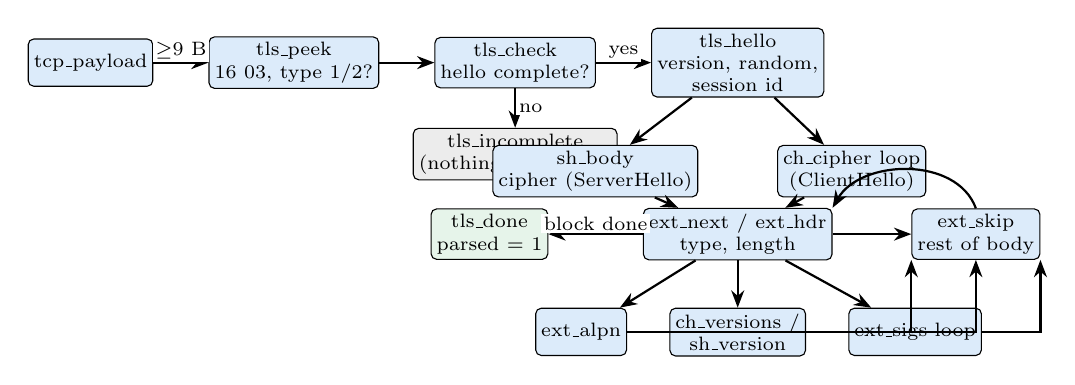
\begin{tikzpicture}[node distance=5mm and 7mm, every node/.style={font=\scriptsize}]
  \tikzset{s/.style={draw, rounded corners=2pt, fill=sw, align=center, inner sep=2pt, minimum height=6mm}}
  \node[s] (pl) {tcp\_payload};
  \node[s, right=of pl] (pk) {tls\_peek\\ 16 03, type 1/2?};
  \node[s, right=of pk] (ck) {tls\_check\\ hello complete?};
  \node[s, below=of ck, fill=gray!15] (inc) {tls\_incomplete\\ (nothing consumed)};
  \node[s, right=of ck] (he) {tls\_hello\\ version, random,\\ session id};
  \node[s, below right=6mm and -6mm of he] (ci) {ch\_cipher loop\\ (ClientHello)};
  \node[s, below left=6mm and -6mm of he] (sh) {sh\_body\\ cipher (ServerHello)};
  \node[s, below=14mm of he] (eb) {ext\_next / ext\_hdr\\ type, length};
  \node[s, below left=6mm and 2mm of eb] (b1) {ext\_alpn};
  \node[s, below=6mm of eb] (b2) {ch\_versions /\\ sh\_version};
  \node[s, below right=6mm and 2mm of eb] (b3) {ext\_sigs loop};
  \node[s, right=10mm of eb] (sk) {ext\_skip\\ rest of body};
  \node[s, left=12mm of eb, fill=ct] (dn) {tls\_done\\ parsed = 1};
  \draw[arr] (pl) -- node[lbl, above]{$\ge$9 B} (pk); \draw[arr] (pk) -- (ck);
  \draw[arr] (ck) -- node[lbl, right]{no} (inc); \draw[arr] (ck) -- node[lbl, above]{yes} (he);
  \draw[arr] (he) -- (ci); \draw[arr] (he) -- (sh);
  \draw[arr] (ci) -- (eb); \draw[arr] (sh) -- (eb);
  \draw[arr] (eb) -- (b1); \draw[arr] (eb) -- (b2); \draw[arr] (eb) -- (b3); \draw[arr] (eb) -- (sk);
  \draw[arr] (b1) -| (sk.south west); \draw[arr] (b2) -| (sk.south); \draw[arr] (b3) -| (sk.south east);
  \draw[arr] (sk.north) to[out=110,in=60] (eb.north east);
  \draw[arr] (eb) -- node[lbl, above]{block done} (dn);
\end{tikzpicture}
\caption{The TLS walk (\code{p4/parser\_tls.p4}), simplified: each loop reads one value per state and returns.}
\end{figure}

\subsection{Forwarding the original bytes: two passes}

\textbf{Problem.} \code{advance} removes the skipped bytes from the packet in BMv2. Extracting a 2,000-byte hello into
headers instead would need a header for every byte, as for the TCP options, and is far too large.

\textbf{Approach.} A packet whose hello was walked is \emph{resubmitted}: BMv2 sends the original packet through the
pipeline again. On that second pass the parser reads only Ethernet (everything else stays payload), and the packet
is forwarded unchanged. The digest was already produced in the first pass. Only packets that start a TLS hello pay
for the second pass (at most one or two per connection).

\subsection{What the switch sends, and what the controller adds}
\label{sec:tls-out}

\begin{figure}[H]\centering
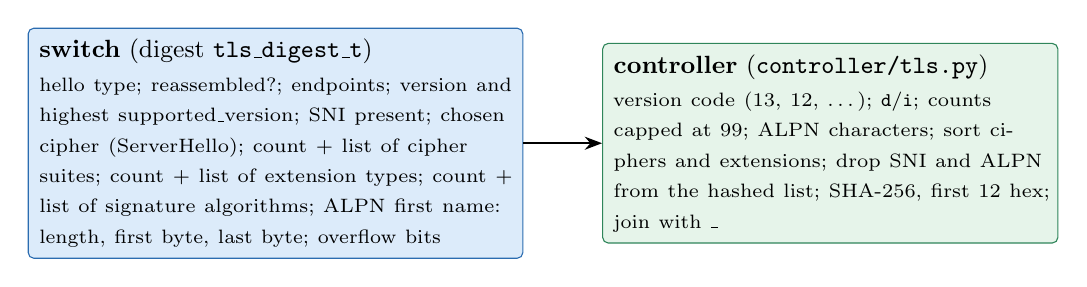
\begin{tikzpicture}[node distance=4mm and 10mm]
  \node[swbox, text width=60mm, align=left] (sw) {\textbf{switch} (digest \code{tls\_digest\_t})\\[1pt]
    \scriptsize hello type; reassembled?; endpoints; version and highest supported\_version; SNI present;
    chosen cipher (ServerHello); count + list of cipher suites; count + list of extension types; count + list of
    signature algorithms; ALPN first name: length, first byte, last byte; overflow bits};
  \node[ctbox, right=of sw, text width=55mm, align=left] (ct) {\textbf{controller} (\code{controller/tls.py})\\[1pt]
    \scriptsize version code (13, 12, \ldots); \code{d}/\code{i}; counts capped at 99; ALPN characters;
    sort ciphers and extensions; drop SNI and ALPN from the hashed list; SHA-256, first 12 hex; join with \code{\_}};
  \draw[arr] (sw) -- (ct);
\end{tikzpicture}
\caption{Division of the JA4/JA4S work. Everything taken from the packet is taken by the switch.}
\end{figure}

\textbf{Why not sort in the switch.} Sorting a list of up to 128 values in P4 needs a sorting network of thousands
of compare-and-swap steps; it is possible but adds nothing to correctness. SHA-256 has no BMv2 primitive at all.

\textbf{Once per connection.} The switch remembers per connection and direction that its hello was reported, so a
retransmitted hello is not reported again.

%=====================================================================
\section{Messages split over packets, out of order, repeated (TLS, HTTP)}
\label{sec:split}

\subsection{The cases}

\begin{itemize}
\item \textbf{Split.} A ClientHello with a post-quantum key share is about 2 KB, more than one segment (Chrome's in
  FoxIO's \code{sigalg-grease.pcapng} arrives as 1,400 + 639 bytes). Any hello can also be cut anywhere by a sender
  or a middlebox, even after its first byte.
\item \textbf{Out of order.} The second segment can arrive before the first (the server's second packet first).
\item \textbf{Repeated / overlapping.} Retransmissions repeat segments; a retransmission can also cover a different
  range than the original.
\item \textbf{Several records.} A hello may be carried in two or more TLS records.
\end{itemize}

\subsection{Why the switch alone cannot do it, and what it does instead}

P4 processes one packet at a time and cannot hold a packet back. Reading a hello across packets would mean storing
the first piece's bytes in registers and resuming the walk in the middle of a list on the next packet, in any
order: a large amount of state and code for an uncommon case. The approach taken keeps every reading in the switch
and moves only the \emph{storage} out:

\begin{enumerate}
\item The switch recognises which segments may belong to a hello that is not complete, and copies them to the
  controller (packet-in), each with its offset in its direction's byte stream.
\item The controller keeps the bytes by offset. When the bytes from the hello's first byte on are contiguous and the
  hello is complete, it takes the hello out of its TLS records and sends it back into the switch as one packet
  (packet-out).
\item The switch walks that packet with the same parser, reports it with the flag \emph{reassembled}, and drops it.
\end{enumerate}
So there is one parser for every hello, whole or joined, and the controller never interprets a field. The same
mechanism serves HTTP requests (Section~\ref{sec:http}) and the certificates of a TLS 1.2 server
(Section~\ref{sec:x509}); the per-direction bookkeeping is the control \code{Stream} (\code{p4/stream.p4}), shared by
all three. The controller learns from a flag on the copy where a message starts and of which type it is (TLS hello,
HTTP request, TLS 1.2 server flight), and follows that type's framing only: TLS records, the empty line that ends an
HTTP header block, the length-prefixed certificate list.

\subsection{Which segments are copied: per-direction state}

The switch keeps, per connection and direction (control \code{Stream}, \code{p4/stream.p4}): the initial sequence
number (from the SYN or SYN-ACK), so that offset = seq $-$ ISN $-$ 1; whether the direction has started (its first
byte seen); whether a message is pending and where it started; the \emph{edge} (the sequence number after the
furthest byte seen) and one gap. A data segment is copied when

\begin{tabularx}{\textwidth}{l X}
\toprule
\textbf{rule} & \textbf{the segment \ldots} \\
\midrule
(a) & starts a message that continues beyond it (an incomplete hello or request; a segment of 1 to 8 bytes that
      begins with \code{0x16} or a method's first letter counts): the message is pending, copied with its type \\
(b) & lies within 16 KB of a pending message's start: a later piece of it \\
(c) & lies within the first 16 KB of a direction that has not started: a piece that arrived before the
      direction's first message \\
(d) & holds a complete TLS 1.2 ServerHello: the server's flight with the certificates starts there (JA4X) \\
(e) & lies ahead of a gap, within 16 KB of it, in a direction that has carried an HTTP request: a piece of the
      next request on a keep-alive connection that arrived before its first segment. The gap opens when a segment
      lands beyond the edge, and closes when a segment covering its first byte arrives (or 16 KB on) \\
\bottomrule
\end{tabularx}

A joined message coming back from the controller clears \emph{pending}. Everything else is forwarded without a copy.
Rule (e) was added after a review of assumptions: a keep-alive connection's second request, cut in two and second
piece first, was never reported (\code{tests/test\_keepalive\_reorder.py}, 18 orders). The same test showed a second
fault: a joined request comes back after the whole requests that followed it, so the connection's JA4H list was out
of order; the HTTP digest now carries the request's sequence number and the controller keeps stream order. Rule (e)
is limited to HTTP directions: in a TLS or SSH connection nothing more is read after the hellos, so copies there
would only be load.

\subsection{The out-of-order case, step by step}

\begin{figure}[H]\centering
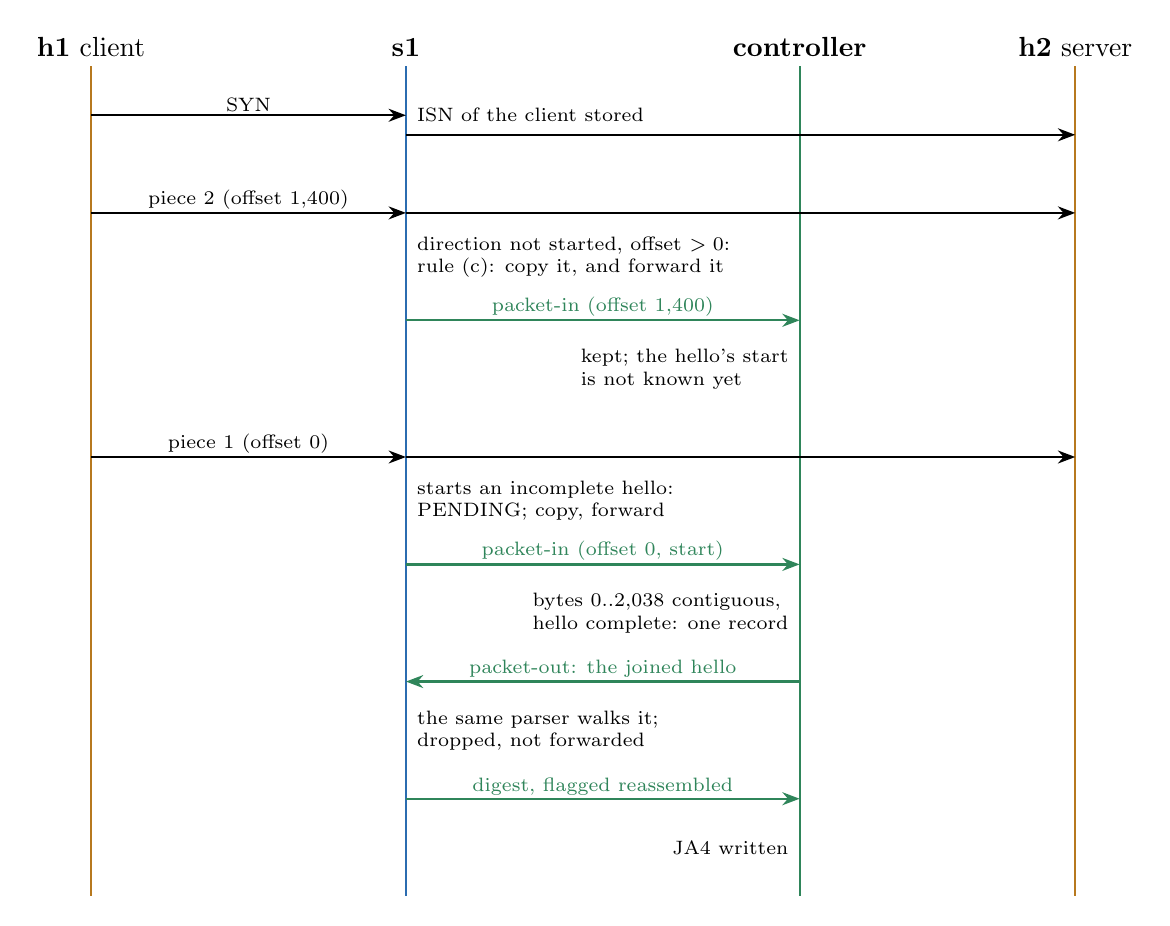
\begin{tikzpicture}[x=1cm,y=-0.62cm]
  \tikzset{note/.style={font=\scriptsize, align=left, fill=white, inner sep=1pt}}
  \draw[thick, hod] (0,0) node[above, black]{\textbf{h1} client} -- (0,17);
  \draw[thick, swd] (4,0) node[above, black]{\textbf{s1}} -- (4,17);
  \draw[thick, ctd] (9,0) node[above, black]{\textbf{controller}} -- (9,17);
  \draw[thick, hod] (12.5,0) node[above, black]{\textbf{h2} server} -- (12.5,17);
  % SYN
  \draw[arr] (0,1) -- node[lbl, above]{SYN} (4,1);
  \node[note, right] at (4.1,1) {ISN of the client stored};
  \draw[arr] (4,1.4) -- (12.5,1.4);
  % piece 2
  \draw[arr] (0,3) -- node[lbl, above]{piece 2 (offset 1,400)} (4,3);
  \node[note, right] at (4.1,3.9) {direction not started, offset $>0$:\\ rule (c): copy it, and forward it};
  \draw[arr] (4,3) -- (12.5,3);
  \draw[arr, ctd] (4,5.2) -- node[lbl, above]{packet-in (offset 1,400)} (9,5.2);
  \node[note, left] at (8.9,6.2) {kept; the hello's start\\ is not known yet};
  % piece 1
  \draw[arr] (0,8) -- node[lbl, above]{piece 1 (offset 0)} (4,8);
  \node[note, right] at (4.1,8.9) {starts an incomplete hello:\\ PENDING; copy, forward};
  \draw[arr] (4,8) -- (12.5,8);
  \draw[arr, ctd] (4,10.2) -- node[lbl, above]{packet-in (offset 0, start)} (9,10.2);
  \node[note, left] at (8.9,11.2) {bytes 0..2,038 contiguous,\\ hello complete: one record};
  % reinject
  \draw[arr, ctd] (9,12.6) -- node[lbl, above]{packet-out: the joined hello} (4,12.6);
  \node[note, right] at (4.1,13.6) {the same parser walks it;\\ dropped, not forwarded};
  \draw[arr, ctd] (4,15) -- node[lbl, above]{digest, flagged reassembled} (9,15);
  \node[note, left] at (8.9,16) {JA4 written};
\end{tikzpicture}
\caption{The second piece of a ClientHello arrives first. Both pieces are forwarded to h2 at once: fingerprinting
never delays traffic.}
\end{figure}

\subsection{Joining in the controller}

\begin{figure}[H]\centering
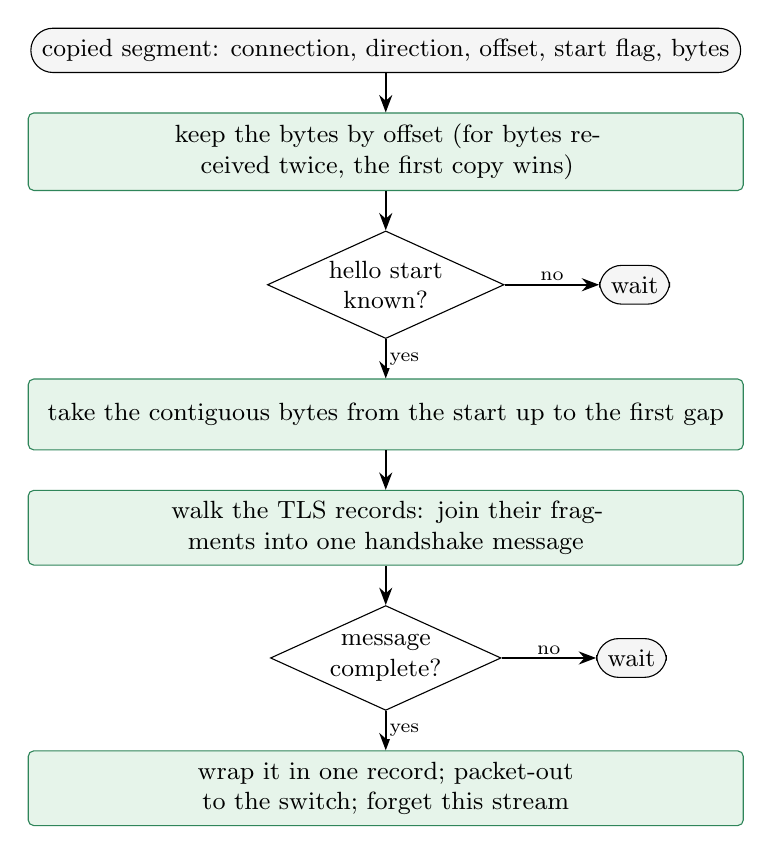
\begin{tikzpicture}[node distance=5mm]
  \node[term] (in) {copied segment: connection, direction, offset, start flag, bytes};
  \node[ctbox, below=of in, text width=88mm] (k) {keep the bytes by offset (for bytes received twice, the first copy wins)};
  \node[dec, below=of k] (st) {hello start\\ known?};
  \node[ctbox, below=of st, text width=88mm] (c) {take the contiguous bytes from the start up to the first gap};
  \node[ctbox, below=of c, text width=88mm] (r) {walk the TLS records: join their fragments into one handshake message};
  \node[dec, below=of r] (cp) {message\\ complete?};
  \node[ctbox, below=of cp, text width=88mm] (o) {wrap it in one record; packet-out to the switch; forget this stream};
  \node[term, right=12mm of st] (w1) {wait};
  \node[term, right=12mm of cp] (w2) {wait};
  \draw[arr] (in) -- (k); \draw[arr] (k) -- (st);
  \draw[arr] (st) -- node[lbl, right]{yes} (c); \draw[arr] (st) -- node[lbl, above]{no} (w1);
  \draw[arr] (c) -- (r); \draw[arr] (r) -- (cp);
  \draw[arr] (cp) -- node[lbl, right]{yes} (o); \draw[arr] (cp) -- node[lbl, above]{no} (w2);
\end{tikzpicture}
\caption{\code{controller/reassembly.py}. It checks only TLS framing (record type and lengths), never a hello
field.}
\end{figure}

\subsection{Tested cases}

\code{tests/test\_split\_reorder.py} takes five real messages: Chrome's 2,039-byte ClientHello, Firefox's 517-byte
ClientHello and a TLS 1.3 ServerHello from FoxIO's captures, FoxIO's HTTP request with cookies, and a browser-like
HTTP request of about 1,700 bytes (40 cookies, Referer, Accept-Language). It cuts them and sends them through the
switch in every case below, each as its own connection. The expected value is FoxIO's, computed on the same message
sent whole in one segment, so the reference never sees the cut. For HTTP the whole list of the connection's JA4H is
compared, so a request reported twice fails too.

\begin{tabularx}{\textwidth}{X r}
\toprule
\textbf{Case} (for each message unless noted) & \textbf{per message} \\
\midrule
two pieces, cut at 1, 4, 5, 6, 9, 10, 43, 44, 100, half, $n-10$, $n-1$ bytes, in order & 12 \\
the same, second piece first & 12 \\
three pieces, all six orders & 6 \\
first piece twice; second piece twice then the first; whole message again after it & 3 \\
overlap (second piece starts 20 bytes early), in order and reversed & 2 \\
one byte per segment, last byte first ($n$ segments) & 1 \\
no SYN seen: two pieces in order, three pieces in order & 2 \\
TLS: after 20 other bytes (as after SOCKS): whole, and split in order & 2 \\
ClientHellos: hello in two TLS records (one segment; split between the records, reversed) & 2 \\
ServerHello: inside a 3,000-byte record with a certificate, cut inside the ServerHello, in order and reversed & 2 \\
\midrule
\textbf{Result: 202 of 202 cases exact} (126 TLS, 76 HTTP) & \\
\textbf{Limit cases, 8 of 8 never wrong} (nothing reported): no SYN and second piece first; after other bytes and second piece first & \\
\bottomrule
\end{tabularx}

\textbf{A bug these tests found.} The first run gave 85 of 112: every cut inside the first 9 bytes failed. Such a
first segment is too short to show the record and handshake headers, so the switch took it as ``not a hello'' and
stopped looking. A first segment of 1 to 8 bytes beginning with \code{0x16} now counts as a possible hello start
and is copied; the controller's framing check decides.

\textbf{The limit, tested too.} Without the SYN the switch learns where the stream starts only from the hello's
first segment, so a piece that arrives before it cannot be placed. The test checks that the switch then reports
nothing, not a wrong value (it reports nothing).

\textbf{The server's side: a TLS 1.2 flight split and out of order.} \code{tests/test\_server\_flight\_reorder.py}
takes h2's flight from the live run (ServerHello, Certificate with a chain of two, ServerKeyExchange,
ServerHelloDone; 2,241 bytes) and sends it as TCP cut it in the live run (1,448 + 793 bytes) in order and second
segment first; as three pieces in all six orders (twice, with different cuts); in 100-byte pieces with the
certificates reversed, and with everything reversed (ServerHello last); duplicated; and overlapping. Copy rule (c)
keeps a certificate piece that arrives before the ServerHello, rule (d) starts the flight at the ServerHello, rule
(b) keeps the pieces after it, and the controller cuts out the certificates once the gap is closed.
\textbf{Result: 19 of 19 exact} (JA4S and both JA4X equal to FoxIO on the flight sent whole). A ServerHello that is
itself split (cut at byte 40, both orders): JA4S exact, JA4X not reported, never wrong (the documented limit).

\textbf{Later requests on a keep-alive connection.} \code{tests/test\_keepalive\_reorder.py}: on one connection a
whole request, then a 1,700-byte request cut into two pieces (cut at 1, 10, 100, half, $n-1$; in order and second
first) or three pieces (all six orders), duplicated or overlapping, then a whole request. Expected: FoxIO's three
JA4H on the requests sent whole, in order. \textbf{Result: 18 of 18 exact} (before rules (e) and the stream order:
0 of 18).

\textbf{Port reuse, VLAN tags, SSH on another port, the controller's memory.} \code{test\_port\_reuse} (two TLS
connections and two SSH sessions, each pair on one four-tuple, one SYN repeated), \code{test\_vlan\_and\_ssh\_port}
(TLS in an 802.1Q tag, HTTP in 802.1ad + 802.1Q, the live SSH session on port 2222) compare every fingerprint with
FoxIO's tool: all exact. \code{test\_controller\_state} checks the reassembler's bounds with a clock passed in, and
the false start inside a request.

%=====================================================================
\section{HTTP fingerprint: JA4H}
\label{sec:http}

\begin{tabularx}{\textwidth}{l X}
\toprule
\multicolumn{2}{l}{\textbf{JA4H} = method version cookie referer \#headers language \code{\_} hash(header names) \code{\_} hash(cookie names) \code{\_} hash(cookie pairs)} \\
method, version & first two letters of the method (\code{ge}, \code{po}, \ldots), \code{10} / \code{11} \\
cookie, referer & \code{c}/\code{n}, \code{r}/\code{n}: a Cookie / Referer header is present \\
\#headers & headers other than Cookie and Referer, two digits \\
language & Accept-Language up to the first \code{,}, without \code{-}, lower case, 4 characters (\code{0} padded) \\
hashes & header names in their order; cookie names and \code{name=value} pairs sorted (the first Cookie header, split at \code{"; "}) \\
\bottomrule
\end{tabularx}

One JA4H per request (FoxIO's tool reports the list of a connection's requests); requests inside TLS (HTTP/2,
HTTP/3) are encrypted and out of reach of a switch.

\textbf{Reading the request in P4.} The request header block is read one byte per parser state, up to the empty line
that ends it: the method's bytes, the last 8 bytes of the request line (the version), every header name, the first
Cookie value split at \code{"; "}, the first Accept-Language value. Header names are compared without regard to case
by setting bit 5 of each byte (the lower case of a letter), which leaves the three names looked for
(\code{cookie}, \code{referer}, \code{accept-language}) exact. A bare LF is accepted wherever CR LF is, as tshark does
(found on FoxIO's \code{http-empty-useragent.pcap}).

\textbf{Strings in a switch.} The digest carries the header names and cookie pairs as byte strings, each item
followed by a zero byte. Two limits of the compiler shaped how they are built:
\begin{itemize}
\item a field may have at most 2,048 bits, so a list is a \emph{chain} of fields (names: 2 fields, 512 bytes;
  cookies: 4 fields, 1,024 bytes) shifted as one register;
\item shifts by a variable amount are limited to 8 bits on BMv2, so every list grows one byte at a time by constant
  bit slices (\code{f1 = f1[2039:0] ++ f0[2047:2040]; f0 = f0[2039:0] ++ b}). A header name goes into the list as
  it is read; when the name turns out to be Cookie or Referer it is taken out again by a constant 6- or 7-byte shift.
\end{itemize}
A list longer than its capacity sets an overflow bit, and the request is reported as incomplete.

\textbf{Retransmissions.} The switch remembers the sequence number of the last request it reported per connection,
so a retransmitted request is not reported twice. Split requests go through the controller's join like hellos:
complete when the joined bytes hold the empty line.

%=====================================================================
\section{SSH fingerprint: JA4SSH}

\textbf{JA4SSH} = \code{c}mode\code{s}mode\code{\_c}\#SSH\code{s}\#SSH\code{\_c}\#ACK\code{s}\#ACK, per window of 200
SSH packets: the most frequent payload length of each side (the smallest on a tie), the number of SSH packets of
each side, the number of bare ACKs of each side. FoxIO's tool counts a segment of an SSH connection with payload as
an SSH packet, and one without payload whose flags are exactly ACK as a bare ACK; when client + server SSH packets reach
200 the window closes and every count restarts; the last, partial window is reported at the end.

\textbf{Before building, the rule was checked.} A 60-line model of this rule was run on FoxIO's SSH captures and
compared with FoxIO's output: equal on every connection except two sample files of deliberately malformed and SSH
version 1 traffic, where tshark refuses a few segments as SSH. (The model first disagreed on \code{ssh2.pcapng}:
it took Ethernet padding of minimum-size frames for payload. The switch computes payload length from the IP header and
cannot make that mistake.)

\begin{figure}[H]\centering
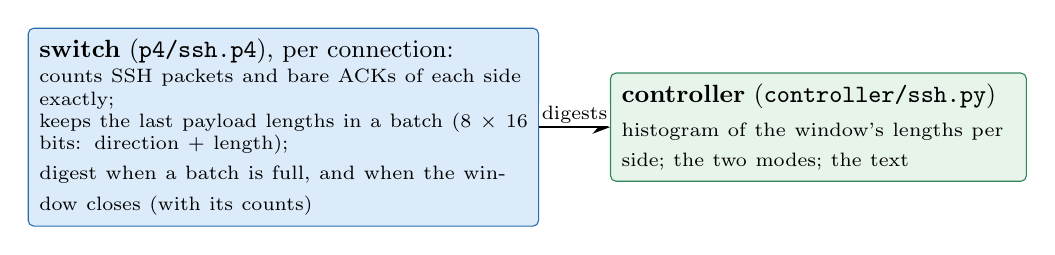
\begin{tikzpicture}[node distance=5mm and 9mm]
  \node[swbox, text width=62mm, align=left] (sw) {\textbf{switch} (\code{p4/ssh.p4}), per connection:\\[1pt]
    \scriptsize counts SSH packets and bare ACKs of each side exactly;\\ keeps the last payload lengths in a batch
    (8 $\times$ 16 bits: direction + length);\\ digest when a batch is full, and when the window closes (with its
    counts)};
  \node[ctbox, right=of sw, text width=50mm, align=left] (ct) {\textbf{controller} (\code{controller/ssh.py})\\[1pt]
    \scriptsize histogram of the window's lengths per side; the two modes; the text};
  \draw[arr] (sw) -- node[lbl, above]{digests} (ct);
\end{tikzpicture}
\caption{JA4SSH: everything is counted in the switch; only the mode, which needs a histogram of up to 200 values, is
computed by the controller.}
\end{figure}

\textbf{The last window.} The reference reports the partial window at the end of its capture. P4Runtime on BMv2
cannot read registers (``Register reads are not supported yet''), so when the traffic is over the controller sends
one small \emph{flush} packet per SSH connection (packet-out kind 2); the switch answers with the connection's
current counts and lengths as a final digest.

\textbf{One digest call.} The flush first had its own \code{digest()} call: that is the per-call-site problem of
Section~4.4 again, so the control was rewritten with a single call.

\textbf{Which connections are SSH.} First only port 22. tshark, under FoxIO's tool, also recognises SSH by its
``SSH-'' banner on any port, so the switch now does too: the parser notes a payload that begins with ``SSH-'', which
marks the connection; on a port other than 22 the client is the side that sent the SYN, and a \emph{start} digest
tells the controller to ask for the connection's last window at the end. The first version gave
\code{c43s43\_c7s6\_c6s6} on port 2222 where FoxIO gives \code{\ldots\_c7s6}: the handshake's ACK comes before the
banner and FoxIO counts it. Bare ACKs are therefore counted from the start of every connection and used once a
banner appears (\code{tests/test\_vlan\_and\_ssh\_port.py}).

%=====================================================================
\section{DHCP fingerprints: JA4D, JA4D6}

FoxIO's open-source command-line tool does not compute JA4D; its Wireshark plugin does (\code{packet-ja4.c}), and its
test data holds the plugin's output for FoxIO's two DHCP captures. That code is the specification here, and that
output the reference (the plugin itself is built for older tshark versions and cannot be loaded on this machine).

\begin{tabularx}{\textwidth}{l X}
\toprule
\multicolumn{2}{l}{\textbf{JA4D} = type size i/n d/n \code{\_} option codes \code{\_} requested codes \quad (one per DHCP message)} \\
type & 5 letters (\code{disco}, \code{offer}, \code{reqst}, \code{dpack}, \ldots; v6: \code{solct}, \code{advrt}, \ldots) \\
size & v4: option 57 (maximum message size); v6: the client DUID's length (option 1); 4 digits, \code{0000} if absent \\
i / n & v4: option 50 (requested IP) present; v6: option 4 (IA\_TA) present \\
d / n & v4: option 81 with a name; v6: option 39 with a name \\
option codes & v4: every option except 0, 50, 53, 81, 255; v6: every option, \emph{including those nested in IA\_NA, IA\_PD, IAADDR, IAPREFIX}, in packet order \\
requested codes & v4: option 55's bytes; v6: option 6's 2-byte codes \\
\bottomrule
\end{tabularx}

\textbf{Nested options without a stack.} DHCPv6 lists options nested inside containers in packet order. The parser
needs no stack for this: when it meets a container it skips only the container's fixed fields (IAID, lifetimes,
address or prefix), so the next bytes it reads are the first sub-option, and the plain linear walk produces exactly
tshark's order.

%=====================================================================
\section{Certificate fingerprint: JA4X}
\label{sec:x509}

\textbf{JA4X} = hash(issuer attribute OIDs) \code{\_} hash(subject attribute OIDs) \code{\_} hash(extension OIDs), per
certificate of the server's chain; each OID written as the hex of its DER content, joined with \code{,} (FoxIO's
\code{ja4x} crate). Only TLS 1.2 and older send the certificates in the clear.

\begin{figure}[H]\centering
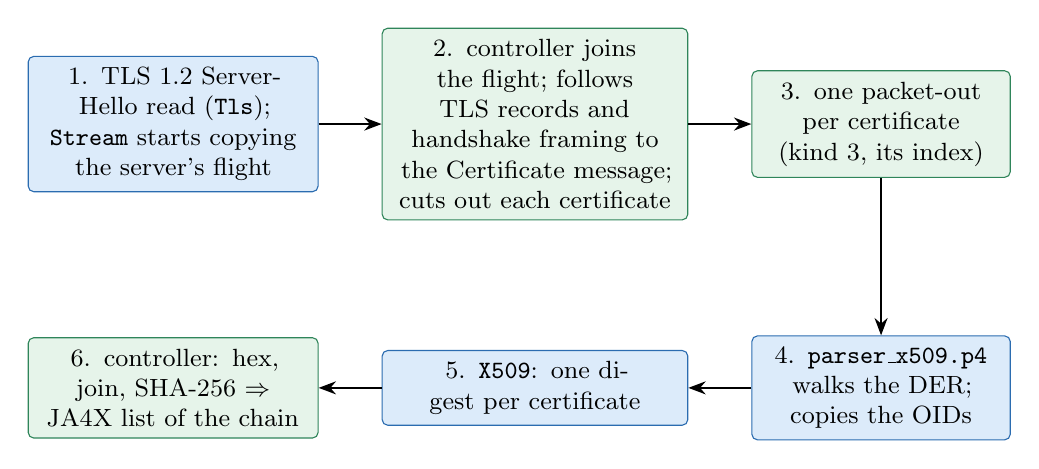
\begin{tikzpicture}[node distance=6mm and 8mm]
  \node[swbox, text width=34mm] (a) {1. TLS 1.2 ServerHello read (\code{Tls});\\ \code{Stream} starts copying\\ the server's flight};
  \node[ctbox, right=of a, text width=36mm] (b) {2. controller joins the flight; follows TLS records and handshake
    framing to the Certificate message; cuts out each certificate};
  \node[ctbox, right=of b, text width=30mm] (c) {3. one packet-out per certificate (kind 3, its index)};
  \node[swbox, below=20mm of c, text width=30mm] (d) {4. \code{parser\_x509.p4} walks the DER; copies the OIDs};
  \node[swbox, left=of d, text width=36mm] (e) {5. \code{X509}: one digest per certificate};
  \node[ctbox, left=of e, text width=34mm] (f) {6. controller: hex, join, SHA-256 $\Rightarrow$ JA4X list of the chain};
  \draw[arr] (a) -- (b); \draw[arr] (b) -- (c); \draw[arr] (c) -- (d); \draw[arr] (d) -- (e); \draw[arr] (e) -- (f);
\end{tikzpicture}
\caption{JA4X. Certificates are long and always span segments, so they always take the join path; the switch reads
every certificate itself.}
\end{figure}

\textbf{Walking DER in a parser.} Every DER element starts with a tag and a length (one byte, or \code{0x8n} and $n$
bytes). One group of states, \code{tlv}, reads that header for every element; a return code
(\code{meta.x509.ret}) says which state continues after it, since a P4 parser has no calls. Each nesting level keeps
a countdown of its remaining bytes (tbsCertificate, Name, RDN set, attribute or extension), so the walk knows where
every SEQUENCE and SET ends without a stack. Each OID's content bytes are copied into the issuer, subject or
extension list as \code{<length><bytes>} (a zero byte can occur inside an OID, so a separator byte would be ambiguous).

%=====================================================================
\section{Capacities: a measurement study}
\label{sec:caps}

The switch keeps every variable-length list in fixed-size fields. A message whose list is longer is reported as
incomplete, never guessed (\code{tests/test\_capacity\_limits.py} sends lists at and one past every capacity). The
capacities were first chosen generously; \code{tools/measure\_field\_counts.py} then measured, over real messages,
how long each list is.

\textbf{Corpus.} FoxIO's 33 sample captures; the live run's capture; captures of earlier work on this machine
(curl-impersonate's Chrome profile, curl); and messages generated here by every client installed: openssl
\code{s\_client} (TLS 1.3 and 1.2), curl (both), wget, Python \code{requests} and \code{urllib}, busybox wget (HTTP only:
it has no TLS) and headless Firefox 157. Each client connects to a local listener that records its first message;
no root needed. Counting is done by tshark (which reassembles split messages) and, for certificates, by Python's
\code{cryptography}: independent of the switch's parser. GREASE values are not counted, as in JA4.

\begin{tabularx}{\textwidth}{X r r r r r r r}
\toprule
\textbf{Quantity} & \textbf{cap} & \textbf{msgs} & \textbf{distinct} & \textbf{p50} & \textbf{p95} & \textbf{p99} & \textbf{max} \\
\midrule
TLS ClientHello cipher suites & 128 & 241 & 132 & 15 & 28 & 46 & 86 \\
TLS ClientHello extensions & 64 & 241 & 132 & 16 & 16 & 18 & 18 \\
TLS ClientHello signature algorithms & 64 & 241 & 132 & 8 & 15 & 20 & 20 \\
TLS ServerHello extensions & 64 & 135 & 27 & 2 & 6 & 6 & 7 \\
HTTP header-name bytes & 512 & 135 & 29 & 51 & 146 & 146 & 146 \\
HTTP cookie bytes & 1,024 & 7 & 7 & 108 & 863 & 863 & 863 \\
DHCP option codes & 64 & 20 & 16 & 5 & 7 & 7 & 7 \\
DHCP requested codes & 128 & 20 & 16 & 0 & 7 & 7 & 7 \\
certificate issuer OID bytes & 256 & 66 & 47 & 16 & 20 & 26 & 26 \\
certificate subject OID bytes & 256 & 66 & 47 & 16 & 26 & 60 & 60 \\
certificate extension OID bytes & 256 & 66 & 47 & 37 & 72 & 72 & 72 \\
\bottomrule
\end{tabularx}

\noindent 1238 of 1238 measured lists (100\%) are within their capacity. ``distinct'': messages counted once per distinct content, so one chatty client does not weigh more. 42 captures; certificates \code{cryptography} could not parse: 0. Source: \code{results/measure/field\_counts.json}.


\textbf{Reading the table.} Every message of the corpus fits. The largest cipher list is 86 suites (FoxIO's
\code{https-connect.pcap}); the clients here send at most 75. Every capacity is above the largest message seen; the closest are
cookies (863 of 1,024 bytes) and cipher suites (86 of 128). Their cost is small on this target: a longer list costs digest bits and parser loop
iterations, not pipeline stages (a sorting network sized to the list, which a Tofino design needs, is not used
here; the controller sorts, Section~\ref{sec:tls-out}). The cookie corpus is small (7 requests with cookies): the
capacity of 1,024 bytes is above the largest seen (863) but real browsers can send more; such a request is reported
incomplete.

%=====================================================================
\section{Problems found and how they were fixed}
\label{sec:problems}

Every error and corner case met while building the project, in one place: what went wrong, how it was found, the
cause and the fix, and what checks it now. Each was found by a test, by the comparison against the reference, or by
the live run, and each fix was checked by rerunning that check. Where a test was written for a bug, it failed on
the old program before the fix and passed after it.

% Shared by design.tex and detailed_architecture.tex: every error and corner case fixed.
% Add a row here for every new fix; both PDFs pick it up.
{\small
\begin{longtable}{>{\raggedright\arraybackslash}p{31mm} >{\raggedright\arraybackslash}p{24mm} >{\raggedright\arraybackslash}p{70mm} >{\raggedright\arraybackslash}p{26mm}}
\toprule
\textbf{What went wrong} & \textbf{Found by} & \textbf{Cause and fix} & \textbf{Checked by} \\
\midrule
\endhead
\bottomrule
\endfoot
\multicolumn{4}{l}{\textit{Reading packets (P4 parser)}} \\[2pt]
MSS 1460 read as 46260 & JA4T vs FoxIO, first comparison & the value was read back through the header stack's \code{.last} after extraction, which gave the wrong bytes. Values are now read with \code{lookahead} before the bytes are extracted & comparison (JA4T 62/62) \\[3pt]
TCP options \code{-0-0} vs \code{-0} & JA4T vs FoxIO & FoxIO lists every padding byte after End-of-Options as another option 0. The walk stopped at EOL; it now treats EOL as a one-byte option and continues & comparison \\[3pt]
two ServerHellos missing & comparison, \code{latest.pcapng} & a hello was required to fill its whole TLS record; servers put ServerHello and Certificate in one long record. Now only the hello itself must be complete ($\mathit{hsLen}+9 \le \mathit{payLen}$ and $\mathit{hsLen}+4 \le \mathit{recLen}$) & comparison \\[3pt]
SOCKS / CONNECT hellos missing & comparison (a regression) & the state ``this stream does not start with a hello'' also stopped the hello from being reported. It now only stops early pieces from being copied & comparison (\code{socks*}, \code{https-connect}) \\[3pt]
a split inside the first 9 bytes not joined & split test: 85 of 112 cases & a first segment shorter than the TLS headers cannot show that a hello starts there. A short segment starting with \code{0x16} (or a method's first letter, for HTTP) now counts as a possible message start and is copied & \code{test\_\allowbreak{}split\_\allowbreak{}reorder} 202/202 \\[3pt]
HTTP request with bare LF line ends & comparison & only CR LF ended a line; FoxIO accepts LF alone. The walk now does too & comparison (JA4H 72/72) \\[3pt]
JA4D6 flag \code{d} for an empty name & live run & \code{udhcpc6} sends option 39 with the flags and a single \code{0x00} (the root, an empty name); ``length $>$ 1'' counted it as a name, FoxIO does not. A name is now present when longer than one byte, or one byte not zero & \code{test\_\allowbreak{}dhcp6\_\allowbreak{}fqdn}; live rerun exact \\[3pt]
lists longer than the switch keeps & measurement study (a path no test exercised) & not a bug: the overflow path had no test. A message one past each capacity is now sent and must be reported incomplete; one at the capacity must equal FoxIO & \code{test\_\allowbreak{}capacity\_\allowbreak{}limits} \\[3pt]
\midrule
VLAN-tagged frames not fingerprinted & review of assumptions; FoxIO's tool reads through tags & the parser went from Ethernet straight to IPv4 / IPv6, so a tagged frame was forwarded with nothing read. Up to two tags are now parsed (802.1Q; 802.1ad outside 802.1Q) and re-emitted & \code{test\_\allowbreak{}vlan\_\allowbreak{}and\_\allowbreak{}ssh\_\allowbreak{}port}: red (6 MISSING), then exact \\[3pt]
SSH on a port other than 22 not fingerprinted & review of assumptions; FoxIO's tool gave JA4SSH on port 2222 & the switch counted port 22 only; tshark recognises SSH by its banner on any port. The parser notes a payload beginning with ``SSH-''; that marks the connection. The first version gave \code{c43s43\_c7s6\_c6s6} for FoxIO's \code{\ldots\_c7s6}: the handshake's ACK comes before the banner and FoxIO counts it. Bare ACKs are now counted from the start of every connection & same test: exact \\[3pt]
\multicolumn{4}{l}{\textit{Compiler and target limits}} \\[2pt]
fields over 2,048 bits; variable shifts & p4c / BMv2 errors & BMv2 fields are at most 2,048 bits, variable shifts at most 8 bits, constant ones 256. Long lists became chains of 2,048-bit fields, grown by constant-width slices & build \\[3pt]
a table applied in two places & p4c error & \code{forward} was applied in each branch; it is now applied once, at the end of ingress & build \\[3pt]
two parser states of the same name & p4c error & the TLS and certificate walks both had \code{ext\_next}; the certificate states became \code{x\_ext\_next}, \code{x\_ext\_read} & build \\[3pt]
\midrule
\multicolumn{4}{l}{\textit{Switch state and digests}} \\[2pt]
JA4L digests before JA4T & digest order in the controller & p4c makes one learn list per \code{digest()} call site, and the controller's settings reached one of them. Every control now has a single call & comparison \\[3pt]
JA4L missing on SSH connections & comparison & BMv2 keeps one digest per packet; the handshake ACK sent JA4L and an SSH start record. The start record was removed and the handshake digest is sent once, after any message digest of the same packet & \code{test\_\allowbreak{}one\_\allowbreak{}digest\_\allowbreak{}per\_\allowbreak{}packet} (red, then green) \\[3pt]
identical messages close together reported once & replay of the live capture & BMv2 drops a digest identical to one not yet acknowledged (Section~\ref{sec:serial}). DHCP, HTTP and SSH digests now carry a serial number & \code{test\_\allowbreak{}identical\_\allowbreak{}digests}: DHCP 3/5 and HTTP 2/6 runs failed before; SSH (with acknowledgements held back) 3/4; all pass after; live rerun: 3+3 identical DHCP messages all reported \\[3pt]
registers not readable over P4Runtime & BMv2 answers UNIMPLE\-MENTED & the last, partial SSH window was to be read from registers. The controller now sends a flush packet; the switch reports the window itself & comparison (JA4SSH) \\[3pt]
\textbf{hello packets not forwarded} & byte-for-byte frame comparison & the second pass (resubmit) lost the arrival port, so \code{forward} missed and the packet was dropped. The port now travels in metadata kept across the resubmit (field list 0) & forwarding check on every run (9,013/9,013) \\[3pt]
copies without their payload & joined messages empty & an ingress copy is parsed again from the start, so the walk consumed its bytes again. Copies are now made at egress (E2E), where the packet is whole & \code{test\_\allowbreak{}split\_\allowbreak{}reorder} \\[3pt]
\midrule
a new connection on reused ports mixed with the old one & review of assumptions; \code{test\_\allowbreak{}port\_\allowbreak{}reuse} & the controller keyed records by endpoints and kept the first value, so the second connection's JA4 was dropped; the SSH counts of two sessions were added together into a \emph{wrong} JA4SSH (\code{c14s12} for \code{c7s6}). Control ConnId now numbers connections (new number on another check or on a SYN with a new sequence number); every control keeps state with it; every TCP digest and copy carries it; the controller keys by it; the previous SSH connection's last window is reported on the new SYN (its handshake digest then goes on a second pass) & \code{test\_\allowbreak{}port\_\allowbreak{}reuse}: red, then every fingerprint of both connections exact \\[3pt]
later request on a keep-alive connection lost when split and out of order & review of assumptions; \code{test\_\allowbreak{}keepalive\_\allowbreak{}reorder} & rule (c) copies early pieces only before a direction has started. Rule (e): the switch keeps each direction's edge and one gap; in a direction that carried an HTTP request, segments ahead of the gap (within 16 KB) are copied until it closes & \code{test\_\allowbreak{}keepalive\_\allowbreak{}reorder} 18/18 \\[3pt]
JA4H of a connection out of order & the same test: every case failed, in order too & a joined request comes back from the controller after the whole requests that followed it; FoxIO lists them in stream order. The HTTP digest now carries the request's sequence number and the controller keeps the list in that order & same test \\[3pt]
\multicolumn{4}{l}{\textit{JA4L (timing)}} \\[2pt]
latency differences of a few ms & comparison with original timing & BMv2 stamps a packet when its pipeline takes it up, not when it arrives; a packet behind a slow walk is stamped late. JA4L is reported as a measurement: TTL scored, latency as a distribution & \code{test\_\allowbreak{}ja4l\_\allowbreak{}gaps} (arithmetic) \\[3pt]
gap test failing now and then & repeated test runs & short gaps were within the 2-CPU VM's scheduling noise; the gaps are now 1\,s and 0.5\,s, checked within 2\% & \code{test\_\allowbreak{}ja4l\_\allowbreak{}gaps} \\[3pt]
\midrule
gap test failing under heavy load & \code{make test} run beside the measurement study (headless Firefox) & BMv2 took the SYN into its pipeline 130\,ms after it was handed over, so the server half was 13\% short; the switch's stamp is the pipeline's, not the arrival's (Section~\ref{sec:testing}). Not changed: the test checks arithmetic and needs an idle machine; a wider tolerance would hide a wrong halving. Passes 3/3 when idle; 6 of 8 with a browser open on the 2-CPU machine (2026-10-12) & \code{test\_ja4l\_\allowbreak{}gaps} \\[3pt]
\midrule
\multicolumn{4}{l}{\textit{Reference and comparison}} \\[2pt]
loopback captures not read & comparison & FoxIO's loopback captures have no Ethernet header; one is added before replay (IPv4 / IPv6 decoded by hand) & comparison \\[3pt]
DHCP inside ICMP errors counted & live run & tshark dissects the DHCP message quoted inside ``port unreachable'' as DHCP; the reference counted four extra messages. It now skips ICMP & equal to FoxIO's plugin output on both samples; live rerun: 10 of 10 DHCP messages exact \\[3pt]
\midrule
reused ports invisible to the comparison & building \code{test\_\allowbreak{}port\_\allowbreak{}reuse} & the references were keyed by endpoints, so a second connection overwrote the first. FoxIO's tool reports tshark's stream number: a later connection on the same endpoints is now keyed with its place among them, the switch's records in the order of their connection numbers & same test (4 JA4T rows, 2 JA4, 2 JA4SSH compared) \\[3pt]
\multicolumn{4}{l}{\textit{Test bench and live run}} \\[2pt]
a stale switch answering a new run & results of an old program & a switch from a stopped run held the fixed gRPC port. Each run takes free ports; the switch dies with its parent (\code{PR\_SET\_PDEATHSIG}) & every run \\[3pt]
packet socket errors & bench start-up failures & a nanomsg socket was opened per send and leaked; a Unix socket path is limited to 107 characters. One socket per run, closed at the end, with a unique short path in the runtime folder & every run \\[3pt]
live run hung on the 2\,KB ClientHello & live run & \code{openssl s\_client -quiet} ignores the end of its input and waited for the time limit. \code{-quiet} removed; \code{timeout -k 2 15} on every client & live rerun completed, every step 0.1--3.3\,s \\[3pt]
Ctrl-C left the network half up & live run & Mininet cannot clean up while a host runs a command; the script now interrupts that command first. \code{dnsmasq} and \code{sshd} were not stopped: every server's process id is now kept & live rerun completed, every step 0.1--3.3\,s \\[3pt]
new flight test: one case failed & first run of \code{test\_\allowbreak{}server\_\allowbreak{}flight\_\allowbreak{}reorder} & a test bug, not a switch bug: in one case the certificate pieces' offsets were not shifted past the ServerHello, so the switch received wrong bytes and (correctly) reported no certificate. Traced by logging every copy the controller received; offsets fixed & 19 of 19 exact \\[3pt]
\code{sshd} would not start & live run preparation & \code{sshd} needs \code{/run/sshd}, made only by the system service. The script creates it & live rerun completed, every step 0.1--3.3\,s \\[3pt]
controller buffers grew without end & review of assumptions & the reassembler kept every copied piece. Now at most 32 KB per direction (lowest offsets dropped first), idle directions dropped after 60 s, at most 100,000 directions & \code{test\_\allowbreak{}controller\_\allowbreak{}state} (red: no limits; then green) \\[3pt]
split/reorder fell to 199 of 202 while bounding the buffers & \code{make test} & my first version also dropped a message's bytes as soon as it was joined. A one-byte segment in the middle of a request that begins like a method (``G'') was ``joined'' as a message first, its bytes dropped, and the real request, whose first segment came last, could not be completed. Early dropping removed; the case is now a unit test & 202/202; \code{test\_\allowbreak{}false\_\allowbreak{}start\_\allowbreak{}inside\_\allowbreak{}a\_\allowbreak{}message} \\[3pt]
live run without JA4H (all rows still EXACT) & live rerun after the connection-number fix & not the switch: h2 answered the three HTTP connections with RST. The script started \code{python3 -m http.server} and waited a fixed 2\,s; the server was not yet listening, and the reference saw the same frames, so nothing was flagged. The script now waits until h2 listens on every server port (up to 30\,s) and checks each client's exit status; a failed step is printed and goes into the results table & final live run: all 9 steps as expected, JA4H exact \\[3pt]
the live DHCP client never got a lease (every live run) & the new exit-status check: DHCP step exit 1 & dnsmasq pings an address and waits about 3\,s before offering it; udhcpc's three tries take 3\,s, so the Offers arrived after it gave up (and h1 answered them with ``port unreachable'', the ICMP-quoted DHCP of an earlier row). Only Discover and Offer were ever exercised. dnsmasq now runs with \code{--no-ping} & final live run: Discover, Offer, Request, ACK, all exact \\[3pt]
\end{longtable}
}


\subsection*{The digest serial number: why 32 bits, and what happens when it wraps}
\label{sec:serial}

\textbf{The cause, in BMv2's code} (\code{behavioral-model/src/bm\_sim/learning.cpp}): every digest is kept in a
\emph{filter} until the controller acknowledges it; a new digest equal, field for field, to one in the filter is
silently dropped (lines 375--376); an acknowledgement removes it (lines 478--492). Two identical DHCP messages (or
two identical HTTP requests on one connection) within the time an acknowledgement takes gave one record.

\textbf{The fix.} One counter register per digest kind (\code{dhcpSerial}, \code{httpSerial}, \code{sshSerial}, one cell each); each
digest carries the counter's value, and the counter goes up by one. One counter for the whole switch, not one per
connection: DHCP has no connection, and nothing more is needed.

\textbf{How many bits.} The serial only has to differ among digests of its kind that are \emph{unacknowledged at the
same time}. That number is about (digest rate) $\times$ (time to acknowledge). The controller acknowledges every
digest list as it receives it; the acknowledgement timeout is set to 1\,s. Even at $10^6$ digests of one kind per
second, held for the whole second, that is below $2^{20}$. So 20 bits suffice, 16 bits ($65{,}536$) would not be safe at
high rates, and 32 bits leave a margin of about $4{,}000\times$, at a cost of 4 bytes per digest (a DHCP digest is
about 420 bytes, an HTTP digest about 1.3\,KB).

\textbf{When it passes $2^{32}-1$.} P4 arithmetic on \code{bit<32>} wraps to 0, a defined behaviour. Wrapping is
harmless and no flag is set: two digests can collide only if the first is still unacknowledged
$4{,}294{,}967{,}296$ digests later \emph{and} all its other fields are equal. The controller never reads the serial
(it does not order or count with it); its only job is to make two digests different, so a wrap flag would carry
nothing to act on.

\textbf{Which digests need it.} DHCP and HTTP: their content can repeat exactly. SSH: its counts start again at
every 200-packet window, so steady traffic (a bulk copy) gives identical windows; on a fast link 200 packets pass
within one acknowledgement time. (A first reading of the code missed this; a test with the acknowledgements held
back showed one window of four lost, and passes with the serial.) Not the others: TLS hellos are reported once per
direction of a connection, certificates once per index, the handshake once per kind per connection.

%=====================================================================
\section{The controller}

\begin{enumerate}
\item Connect to the switch over gRPC and become the primary controller (P4Runtime arbitration).
\item Load the compiled program (\code{build/main.json}, \code{build/main.p4info.txtpb}).
\item Install forwarding (port 1 $\leftrightarrow$ 2) and the copy session (clone session 100 $\rightarrow$ CPU port
  255, so copies arrive as packet-in).
\item Enable the six digests (handshake, TLS, HTTP, SSH, DHCP, certificate) with ``send immediately, one per
  message''; acknowledge every digest list (BMv2 drops a digest identical to one not yet acknowledged; the
  DHCP, HTTP and SSH digests carry a serial number for this reason, Section~\ref{sec:serial}).
\item Digest: find the connection's record (the same key from either direction, and the connection's number),
  write the fingerprint text, print it, keep it. A connection's JA4H are kept in stream order (each HTTP digest
  carries its request's sequence number). Packet-in: hand the segment to the reassembler; a joined message (or the certificates of a server
  flight) goes back as packet-out.
\item Finish: one SSH flush per SSH connection, wait for the final windows, write all records as JSON.
\end{enumerate}
The reassembler's memory is bounded: at most 32 KB per direction (lowest offsets dropped first), a direction idle
for 60\,s is dropped, at most 100,000 directions (\code{tests/test\_controller\_state.py}). A first version also
dropped a message's bytes as soon as it was joined; that broke 3 of the 202 split cases (a one-byte segment inside a
request that begins like a method is ``joined'' first, and the real request then lacks its bytes) and was removed.

%=====================================================================
\section{Testing against the reference}
\label{sec:testing}

\begin{figure}[H]\centering
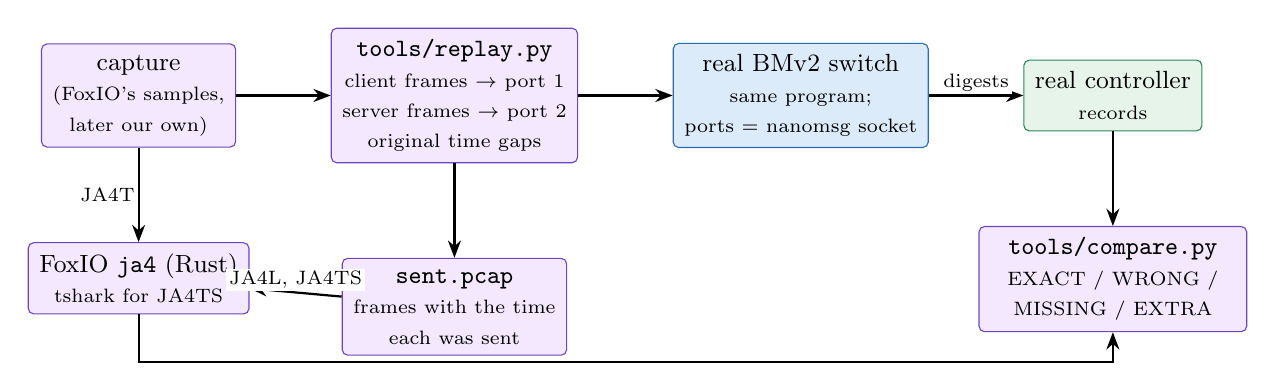
\begin{tikzpicture}[node distance=8mm and 12mm]
  \node[rfbox] (pcap) {capture\\ \scriptsize (FoxIO's samples,\\ \scriptsize later our own)};
  \node[rfbox, right=of pcap] (rp) {\code{tools/replay.py}\\ \scriptsize client frames $\to$ port 1\\ \scriptsize server frames $\to$ port 2\\ \scriptsize original time gaps};
  \node[swbox, right=of rp] (s) {real BMv2 switch\\ \scriptsize same program;\\ \scriptsize ports = nanomsg socket};
  \node[ctbox, right=of s] (c) {real controller\\ \scriptsize records};
  \node[rfbox, below=12mm of rp] (sent) {\code{sent.pcap}\\ \scriptsize frames with the time\\ \scriptsize each was sent};
  \node[rfbox, below=12mm of pcap] (ref) {FoxIO \code{ja4} (Rust)\\ \scriptsize tshark for JA4TS};
  \node[rfbox, below=12mm of c, minimum width=34mm] (cmp) {\code{tools/compare.py}\\ \scriptsize EXACT / WRONG /\\ \scriptsize MISSING / EXTRA};
  \draw[arr] (pcap) -- (rp); \draw[arr] (rp) -- (s); \draw[arr] (s) -- node[lbl, above]{digests} (c);
  \draw[arr] (rp) -- (sent);
  \draw[arr] (pcap) -- node[lbl, left]{JA4T} (ref);
  \draw[arr] (sent) -- node[lbl, above, align=center]{JA4L, JA4TS} (ref);
  \draw[arr] (c) -- (cmp);
  \draw[arr] (ref.south) |- ++(0,-6mm) -| (cmp.south);
\end{tikzpicture}
\caption{The test bench: no root, the real switch, the real controller, an independent reference.}
\end{figure}

\textbf{References}, all independent of this project:
\begin{itemize}
\item FoxIO's Rust tool \code{ja4}: JA4T, JA4L, JA4, JA4S, JA4H, JA4SSH, JA4X;
\item tshark's fields for JA4TS (the open-source tool does not compute it), written in the JA4T format;
\item FoxIO's Wireshark plugin's own test output for JA4D / JA4D6 on FoxIO's two DHCP captures; for traffic captured
  here, the same computation from tshark's fields (\code{tools/reference.py}, equal to the plugin's output on both
  samples). It skips DHCP messages quoted inside ICMP errors: tshark dissects the quoted copy as DHCP, but it is not a
  DHCP message on the wire (the live run's ``port unreachable'' replies quote the server's offers).
\end{itemize}

\textbf{Connections} are matched by their endpoints and, for a later TCP connection on the same endpoints (port
reuse), by their place among them: in the reference from tshark's stream numbers (which FoxIO's tool reports), on
the switch's side in the order of the connection numbers.

\textbf{Verdicts.} Each fingerprint of each connection is EXACT, WRONG, MISSING (only the reference has it) or EXTRA
(only the switch has it). A difference checked by hand, where the reference cannot see what the switch reports, is
EXPLAINED, with the reason written next to it in \code{tools/compare.py}. Not compared, and counted separately:
captures with tunnels (the switch reads only outer headers), QUIC, and HTTP/2 / TLS 1.3 values that FoxIO's tool
could compute only by decrypting with keys stored in the capture.

\textbf{Forwarding.} Every frame sent into the switch must come out, byte for byte unchanged; a run with a lost or
altered frame fails. (This check was added after it found the hello packets that were not forwarded.)

\textbf{JA4L} is a measurement. The TTL part is scored like any fingerprint. The latency is compared with the
reference run on the frames as the replay sent them (\code{sent.pcap}) and reported as a distribution, not
EXACT/WRONG: BMv2 stamps a packet when its ingress pipeline takes it up, so a packet waiting behind a slower one (a
TLS hello walk) is stamped late, by up to a few milliseconds on this 2-CPU virtual machine. The arithmetic is
checked exactly by \code{tests/test\_ja4l\_gaps.py}: a crafted handshake with gaps of 1 s and 0.5 s, against the
send times, within 2\% (a wrong halving or a swapped timestamp would be off by 50--100\%).

\textbf{Captures that are not Ethernet} (FoxIO's loopback captures) get an Ethernet header before replay.

\subsection*{Results}
\begin{center}\begin{tabular}{lrrrrr}\toprule
\textbf{Fingerprint} & \textbf{EXACT} & \textbf{EXPLAINED} & \textbf{WRONG} & \textbf{MISSING} & \textbf{EXTRA}\\\midrule
JA4T & 62 & 0 & 0 & 0 & 0\\
JA4TS & 51 & 0 & 0 & 0 & 0\\
JA4L-C (TTL) & 51 & 0 & 0 & 0 & 0\\
JA4L-S (TTL) & 51 & 0 & 0 & 0 & 0\\
JA4 & 152 & 0 & 0 & 0 & 0\\
JA4S & 92 & 1 & 0 & 0 & 0\\
JA4H (per connection) & 72 & 0 & 0 & 0 & 0\\
JA4SSH (per connection) & 6 & 4 & 0 & 0 & 0\\
JA4X (per chain) & 26 & 0 & 0 & 0 & 0\\
JA4D / JA4D6 (per message) & 10 & 0 & 0 & 0 & 0\\
\midrule Total & 573 & 5 & 0 & 0 & 0\\\bottomrule\end{tabular}\end{center}
All 33 of FoxIO's sample captures that hold traffic the switch reads, replayed with their original timing; 3 tunnel captures excluded. \textbf{Forwarding: 9,013 of 9,013 frames left the switch byte for byte unchanged.} JA4L latency (a measurement, see above), difference to the reference over the same frames: median 331~µs, 90th percentile 1341~µs, maximum 4759~µs (2 of the halves above 2~ms). Not compared: 16 JA4H of HTTP/2 requests and 3 JA4X of TLS~1.3 certificates that FoxIO's tool could compute only by decrypting with keys stored in the captures. The 5 EXPLAINED: one SOCKS4 ServerHello the reference cannot decode (checked by hand), four JA4SSH of malformed or SSH~v1 streams where tshark refuses a few segments as SSH. Source: \texttt{results/compare\_all.json}.


%=====================================================================
\section{Live run: h1 -- s1 -- h2 in Mininet}
\label{sec:live}

The comparison above replays captures. The live run checks the same switch and controller on a real network with
real programs: \code{network/run\_live.py} (root, for Mininet's network namespaces).

\begin{figure}[H]\centering
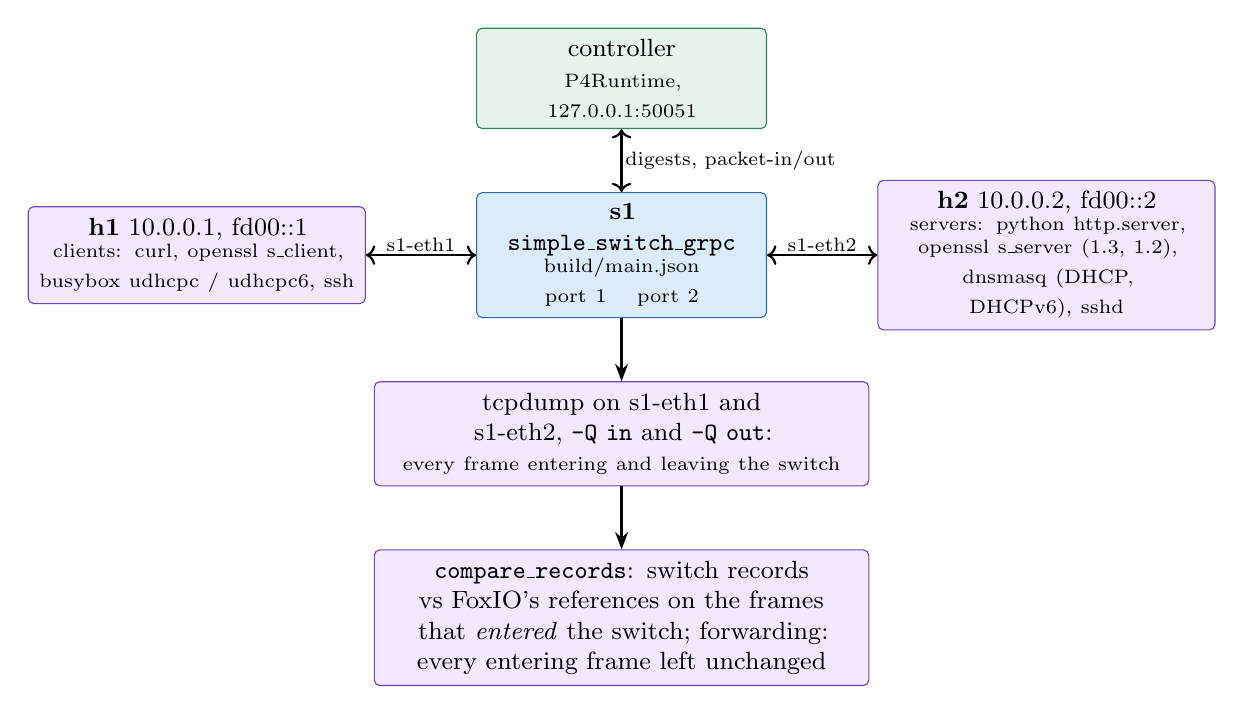
\begin{tikzpicture}[node distance=8mm and 14mm]
  \node[rfbox, text width=40mm] (h1) {\textbf{h1} 10.0.0.1, fd00::1\\ \scriptsize clients: curl, openssl s\_client,\\ \scriptsize busybox udhcpc / udhcpc6, ssh};
  \node[swbox, right=of h1, text width=34mm] (s1) {\textbf{s1}\\ \code{simple\_switch\_grpc}\\ \scriptsize build/main.json\\ \scriptsize port 1 \quad port 2};
  \node[rfbox, right=of s1, text width=40mm] (h2) {\textbf{h2} 10.0.0.2, fd00::2\\ \scriptsize servers: python http.server,\\ \scriptsize openssl s\_server (1.3, 1.2),\\ \scriptsize dnsmasq (DHCP, DHCPv6), sshd};
  \node[ctbox, above=of s1, text width=34mm] (c) {controller\\ \scriptsize P4Runtime, 127.0.0.1:50051};
  \node[rfbox, below=of s1, text width=60mm] (cap) {tcpdump on s1-eth1 and s1-eth2, \code{-Q in} and \code{-Q out}:\\ \scriptsize every frame entering and leaving the switch};
  \node[rfbox, below=of cap, text width=60mm] (cmp) {\code{compare\_records}: switch records vs FoxIO's references on the frames that \emph{entered}
    the switch; forwarding: every entering frame left unchanged};
  \draw[arr, <->] (h1) -- node[lbl, above]{s1-eth1} (s1); \draw[arr, <->] (s1) -- node[lbl, above]{s1-eth2} (h2);
  \draw[arr, <->] (c) -- node[lbl, right]{digests, packet-in/out} (s1);
  \draw[arr] (s1) -- (cap); \draw[arr] (cap) -- (cmp);
\end{tikzpicture}
\caption{The live run. Offloads (TSO, GSO, GRO, checksum) are off on every interface, so the frames are what a real
network carries: TCP itself splits the large messages.}
\end{figure}

\begin{tabularx}{\textwidth}{l X l}
\toprule
\textbf{Step (h1)} & \textbf{What it exercises} & \textbf{Fingerprints} \\
\midrule
HTTP GET & a plain request & JA4T, JA4TS, JA4L, JA4H \\
HTTP with cookies & Cookie, Referer, Accept-Language & JA4H (all four parts) \\
HTTP request of 3\,KB & a request TCP splits over three segments: the join path & JA4H \\
TLS 1.3 & ClientHello and ServerHello & JA4, JA4S \\
TLS 1.2 & the certificate flight in the clear, a chain of two & JA4, JA4S, JA4X ($\times$2) \\
ClientHello of 2\,KB & a hello TCP splits over two segments: the join path & JA4 \\
DHCP & Discover, Offer, Request, ACK (a lease is obtained) & JA4D \\
DHCPv6 & Solicit, Advertise, Request, Reply & JA4D6 \\
SSH & key exchange, a refused login & JA4SSH \\
\bottomrule
\end{tabularx}

\subsection*{What the first live run found}
\begin{enumerate}
\item \textbf{JA4D6 domain flag} (a switch bug): \code{udhcpc6}'s empty name in option 39 was counted as a name.
  Fixed in \code{parser\_dhcp.p4}; see the table of problems.
\item \textbf{DHCP inside ICMP errors} (a reference bug): h1 answered the server's offers with ``port unreachable'',
  which quote the offer; tshark dissects the quote as DHCP and the reference counted four extra messages. The
  reference now skips them.
\item \textbf{Identical messages close together} (a switch bug), found replaying the live capture: three identical
  Offers 0.1\,ms apart gave two records. Fixed with a serial number in the DHCP, HTTP and SSH digests.
\end{enumerate}

\subsection*{The runs after the fixes}
\textbf{First rerun} (after the three fixes above): 49 of 49 exact, 196 of 196 frames unchanged. The three identical
Discovers and the three identical Offers were each reported (the serial number), the DHCPv6 Solicit and Request
carry \code{n}, and the reference counts 10 DHCP messages, not 14.

\textbf{After the connection number and the other fixes of the assumptions review}, two faults of the run script
showed. (1) One run had no JA4H while every row was still EXACT: \code{http.server} was not yet listening after the
fixed 2\,s pause, h2 answered the HTTP connections with RST, and the reference saw the same frames. The script now
waits until h2 listens on every server port and checks every client's exit status. (2) That check then showed that
the DHCP client had never obtained a lease in any live run: dnsmasq pings an address and waits about 3\,s before
offering it, and udhcpc gave up after its 3\,s of tries, so only Discover and Offer had been exercised (and h1's
``port unreachable'' answers to the late Offers were the ICMP-quoted DHCP of the first run). dnsmasq now runs with
\code{--no-ping}.

\textbf{The final run} (below): all 9 steps ended as expected, every fingerprint matched FoxIO (47 of 47), and all
182 frames that entered the switch left it unchanged. DHCP now goes Discover, Offer, Request, ACK, adding
\code{reqst} and \code{dpack} to the messages checked live. Two things in the console output are expected, not
faults: for the split ClientHello, JA4S is printed before JA4 (the ServerHello arrives whole, while the hello waits
for its second segment and the join), and the 3\,KB request's JA4H appears after the step ends (the controller joins
it as the last segment arrives). Identical messages close together no longer occur in the live run; they are
covered by \code{test\_identical\_digests}.

\subsection*{Results}
\begin{center}\begin{tabular}{lrrrrr}\toprule
\textbf{Fingerprint} & \textbf{EXACT} & \textbf{EXPLAINED} & \textbf{WRONG} & \textbf{MISSING} & \textbf{EXTRA}\\\midrule
JA4T & 7 & 0 & 0 & 0 & 0\\
JA4TS & 7 & 0 & 0 & 0 & 0\\
JA4L-C (TTL) & 7 & 0 & 0 & 0 & 0\\
JA4L-S (TTL) & 7 & 0 & 0 & 0 & 0\\
JA4 & 3 & 0 & 0 & 0 & 0\\
JA4S & 3 & 0 & 0 & 0 & 0\\
JA4H (per connection) & 3 & 0 & 0 & 0 & 0\\
JA4SSH (per connection) & 1 & 0 & 0 & 0 & 0\\
JA4X (per chain) & 1 & 0 & 0 & 0 & 0\\
JA4D / JA4D6 (per message) & 8 & 0 & 0 & 0 & 0\\
\midrule Total & 47 & 0 & 0 & 0 & 0\\\bottomrule\end{tabular}\end{center}
One live run of \code{network/run\_live.py}, compared on the frames that entered the switch. \textbf{Forwarding: s1-eth1 $\to$ s1-eth2: 95 of 95; s1-eth2 $\to$ s1-eth1: 85 of 85 frames left the switch unchanged.} JA4L latency (a measurement), difference to the reference over the same frames: 14 halves, median 23~µs, maximum 73~µs. Source: \texttt{results/live/rows.json}.


%=====================================================================
\section{Assumptions, and what changes on a real network}
\label{sec:assumptions}

What the design assumes, why it holds on h1 -- s1 -- h2, and what a real network changes. Rows marked
\textbf{fixed} were found by this review and fixed (the problems table has each fix and its test).

% Shared by design.tex and detailed_architecture.tex: what the project assumes, why it holds on h1 -- s1 -- h2, and
% what changes on a real network. Every new assumption or deployment note goes here.
{\small
\begin{longtable}{>{\raggedright\arraybackslash}p{30mm} >{\raggedright\arraybackslash}p{34mm} >{\raggedright\arraybackslash}p{46mm} >{\raggedright\arraybackslash}p{40mm}}
\toprule
\textbf{Assumption} & \textbf{Holds here because} & \textbf{On a real network} & \textbf{Status} \\
\midrule
\endhead
\bottomrule
\endfoot
\multicolumn{4}{l}{\textit{Where the switch sits}} \\[2pt]
both directions of a connection pass through the switch & one path between h1 and h2 & with asymmetric routing (ECMP, several uplinks) one switch may see one direction: JA4TS, JA4L, JA4S, JA4SSH and the server-side join need the other & a deployment requirement: place the switch where both directions pass (an access or edge link) \\[3pt]
one switch fingerprints a connection & one switch & several P4 switches on a path would each report the same connection & a deployment choice: one fingerprinting point per path, or deduplicate in the controller by endpoints and time \\[3pt]
JA4L measures from the switch & the switch is between h1 and h2 & JA4L-C is switch$\leftrightarrow$client, JA4L-S switch$\leftrightarrow$server: the values depend on where the switch is (FoxIO measures at the server) & correct for an observer in the path; stated with the results \\[3pt]
\multicolumn{4}{l}{\textit{Identifying connections and roles}} \\[2pt]
endpoints identify a connection & every run used fresh ports & clients and NATs reuse ports & \textbf{fixed}: a connection number (ConnId, D21); \code{test\_port\_reuse} \\[3pt]
the client is the SYN sender & every connection starts with a SYN in the captures & a capture or a switch that starts mid-connection sees no SYN & the ClientHello or request sender is then the client; for SSH on port 22 the port; tested without the SYN (limit cases never wrong) \\[3pt]
SSH runs on port 22 & sshd listened on 22 & SSH on other ports is common & \textbf{fixed}: recognised by its banner, as FoxIO's tool does (D23) \\[3pt]
frames are untagged & Mininet's links carry no VLANs & access and trunk links carry 802.1Q / 802.1ad tags & \textbf{fixed}: up to two tags (D23); more: forwarded, not fingerprinted \\[3pt]
two connections never share a slot & a few connections per run & with many connections, two can hash to the same of 65,536 slots & detected by the 32-bit check (never mixed); the older loses its remaining state; slots are one constant \\[3pt]
the same addresses are not in use in two VLANs & one network & overlapping address spaces in different VLANs give the same slot & the VLAN id is not part of the key: a one-line change if needed \\[3pt]
\multicolumn{4}{l}{\textit{Load and memory}} \\[2pt]
split messages are uncommon & most test messages fit in a segment & current Chrome and Firefox ClientHellos carry post-quantum key shares (about 2 KB) and are always split: on browser traffic the controller's join is the common path for JA4 & correctness unaffected (the switch still reads every byte); the controller path's throughput is part of the performance evaluation \\[3pt]
the controller's state fits in memory & runs of seconds & runs of days & \textbf{fixed} for the reassembler (D24); records are kept until the run ends and written as JSON: a long-running deployment exports and drops them \\[3pt]
the machine is idle & tests run alone & BMv2 is software: a busy CPU delays pipeline pick-up, which JA4L measures & JA4L reported as a measurement; the gap test needs an idle machine; hardware stamps on arrival \\[3pt]
\multicolumn{4}{l}{\textit{The target}} \\[2pt]
the program runs on BMv2 (v1model) & BMv2 is the software target & a hardware target (Tofino) would not compile it as written: parser loops over hundreds of bytes, \code{advance}, resubmit for every walked packet, 2,048-bit fields, 16 KB windows & the claim is fingerprinting in a P4 data plane on a software target; a hardware port is a separate design \\[3pt]
only h1 and h2 send into the switch & Mininet's links & the switch's interfaces (s1-eth1, s1-eth2) live in the VM's own network namespace, so the VM's operating system also sends frames on them (IPv6 neighbour discovery, multicast listener reports, mDNS); the switch takes them in and forwards them like any frame (seen in a live run with the switch's trace log: 30 such frames) & harmless here (nothing the switch fingerprints); on a real switch only the cables' traffic arrives \\[3pt]
forwarding is port 1 $\leftrightarrow$ port 2 & two hosts & a real switch forwards by MAC or IP tables & independent of fingerprinting: the \code{forward} table can be any forwarding \\[3pt]
\end{longtable}
}


%=====================================================================
\section{What is done, what is not, and why}
\label{sec:coverage}
% Shared by design.tex and detailed_architecture.tex: what is done, what is not, and why not.
% Keep it in step with every change: a gap closed moves from the second table to the first.

\textbf{The claim the evidence supports.} For clear-text TCP and DHCP traffic through the switch, every JA4+
fingerprint that can be computed passively without keys (JA4, JA4S, JA4H, JA4X, JA4T, JA4TS, JA4L, JA4SSH, JA4D,
JA4D6) is computed in the P4 data plane and matches FoxIO's own tools, for messages whole, split, reordered,
duplicated or overlapping, sent by the client or by the server. The project does \emph{not} claim that
fingerprinting is complete in every respect: the second table lists what is missing and why.

\subsubsection*{Done, and the evidence}
{\small
\begin{longtable}{>{\raggedright\arraybackslash}p{24mm} >{\raggedright\arraybackslash}p{40mm} >{\raggedright\arraybackslash}p{24mm} >{\raggedright\arraybackslash}p{60mm}}
\toprule
\textbf{Fingerprint} & \textbf{FoxIO's samples} (exact / explained) & \textbf{final live run} & \textbf{tests} \\
\midrule
\endhead
\bottomrule
\endfoot
JA4T, JA4TS & 62, 51 & 7, 7 & split / reorder bench; port reuse; VLAN; one digest per packet \\
JA4L (C, S) & TTL 51 / 51; latency as a measurement (median 331\,µs off the reference) & 7, 7 & \code{test\_ja4l\_gaps} (1\,s and 0.5\,s gaps, within 2\,\%; needs an idle machine) \\
JA4 & 152 & 3 (one hello split by TCP) & 202 split / reorder cases; capacity edges; port reuse; VLAN \\
JA4S & 92 / 1 & 3 & split / reorder (ServerHello); server flight in 19 orders \\
JA4H & 72 (per connection) & 3 (one 3\,KB request split by TCP) & split / reorder (HTTP); keep-alive in 18 orders; capacity; identical requests; two VLAN tags \\
JA4X & 26 (per chain) & 1 chain of 2 & server flight in 19 orders \\
JA4SSH & 6 / 4 & 1 & identical windows; port reuse; SSH on port 2222 \\
JA4D, JA4D6 & 10 & 8 (Discover, Offer, Request, ACK; Solicit, Advertise, Request, Reply) & identical messages; DHCPv6 empty name; capacity \\
\midrule
forwarding & 9,013 / 9,013 frames unchanged & 182 / 182 & every replay test \\
\end{longtable}
}

\clearpage
\subsubsection*{Not done, or not proven, and why}
{\small
\begin{longtable}{>{\raggedright\arraybackslash}p{32mm} >{\raggedright\arraybackslash}p{28mm} >{\raggedright\arraybackslash}p{50mm} >{\raggedright\arraybackslash}p{38mm}}
\toprule
\textbf{What} & \textbf{Effect} & \textbf{Why it is not done} & \textbf{What doing it would take} \\
\midrule
\endhead
\bottomrule
\endfoot
\multicolumn{4}{l}{\textit{Fingerprints not implemented}} \\[2pt]
JA4 over QUIC (\code{q\ldots}), the client's HTTP/3 & no JA4 for HTTP/3 browser traffic, a large share of real traffic & the scope set for the project is TCP and DHCP. QUIC carries the ClientHello in Initial packets protected with keys derived from public values (HKDF over the connection id, AES-GCM, header protection): readable passively, so FoxIO computes it, but v1model has no AES or HKDF, so the P4 pipeline cannot decrypt & the controller decrypts the Initial packets and sends the CRYPTO frames back for the same TLS parser (as joined messages are now); a scope decision for the faculty \\[3pt]
JA4 over DTLS (\code{d\ldots}) & no JA4 for DTLS (WebRTC, VPNs) & not in the scope; not in the test traffic & a DTLS record parser in front of the TLS walk (clear hellos, no decryption) \\[3pt]
JA4TScan & -- & an \emph{active} fingerprint (it sends probes); a switch that observes traffic does not probe & not applicable \\[3pt]
\multicolumn{4}{l}{\textit{Traffic not read}} \\[2pt]
tunnels (GRE, VXLAN, Geneve) & inner connections forwarded, not fingerprinted; 3 FoxIO captures excluded & not in the scope (no tunnels on h1 -- s1 -- h2) & a second parser path for the inner headers, the key on the inner endpoints \\[3pt]
IPv6 extension headers & such packets forwarded, not fingerprinted & none in the test traffic; not yet written & a parser loop over the extension headers (hop-by-hop, routing, destination options, first fragment) \\[3pt]
more than two VLAN tags & forwarded, not fingerprinted & not used on access links & one more parser state per tag \\[3pt]
encrypted content: HTTP/2, HTTP/3 requests, TLS 1.3 certificates & no JA4H / JA4X there & impossible without the session keys; FoxIO computes them only from captures that store the keys (16 JA4H and 3 JA4X not compared) & not possible on the wire \\[3pt]
\multicolumn{4}{l}{\textit{Documented limits (the value is missing, never wrong; each one tested)}} \\[2pt]
a piece before its message's first segment, no SYN seen & that message not reported & without the SYN the offset of an early piece is unknown, so it cannot be placed & not possible without the SYN \\[3pt]
a TLS hello after other bytes (SOCKS), split and out of order & not reported & rule (e) covers HTTP directions only; copying after every gap in TLS connections would be load for a rare case & extend (e) to a direction whose first message was not a hello \\[3pt]
a TLS 1.2 ServerHello itself split & no JA4X for that flight & the certificate copy starts at a ServerHello that is complete in one segment; a ServerHello is about 100 bytes, so this is rare & start the flight copy when the joined ServerHello comes back \\[3pt]
two connections in one slot at once & the older loses its remaining state & 65,536 hashed slots, detected by the 32-bit check & more slots (one constant) or buckets \\[3pt]
lists longer than the capacities & reported ``incomplete'' & fixed-size fields in P4; measured: 1,238 of 1,238 lists in 42 captures fit & larger fields (cost: metadata and digest size) \\[3pt]
\multicolumn{4}{l}{\textit{Not tested, so not proven}} \\[2pt]
several Cookie headers in one request & the switch uses the first one's pairs; FoxIO's behaviour not checked & no sample has it & a test against FoxIO's tool \\[3pt]
a second ClientHello after a TLS 1.3 HelloRetryRequest & the switch reports the first only (once per direction); FoxIO's behaviour not checked & no sample has it & a test against FoxIO's tool \\[3pt]
\multicolumn{4}{l}{\textit{Measurement and evidence}} \\[2pt]
JA4L on BMv2 & the time is stamped when the pipeline takes the packet up; on a busy CPU that is late & a property of the software target, not of the program; the TTL part is exact & a hardware target stamps on arrival \\[3pt]
the corpus & FoxIO's 33 sample captures, the live runs and generated cases, not a large real-world capture & evaluation is the next phase of the project & a real-traffic evaluation (planned) \\[3pt]
\multicolumn{4}{l}{\textit{Deployment (not fingerprinting bugs; see the assumptions table)}} \\[2pt]
both directions through one switch; one fingerprinting point; BMv2 only & see the assumptions table & properties of where the switch is placed and of the target & placement rules; a hardware port is a separate design \\[3pt]
\end{longtable}
}


%=====================================================================
\section{Known limits}
\begin{itemize}
\item IPv6 extension headers between the IPv6 header and TCP/UDP are not walked: such packets are forwarded but not
  fingerprinted. Tunnels (GRE, VXLAN, Geneve) are not opened. Up to two VLAN tags are read; a frame with more is
  forwarded, not fingerprinted.
\item Two connections that hash to the same register slot at the same time: the newer one takes the slot; the older
  one loses its remaining state.
\item Capacities, beyond which a fingerprint is reported as incomplete, never guessed: TLS 128 cipher suites, 64
  extensions, 64 signature algorithms; HTTP 512 bytes of header names, 1,024 bytes of cookies; DHCP 64 options, 128
  requested codes; certificates 256 bytes per OID list. A split message is joined only within its first 16 KB.
\item Without the SYN, a piece of a message that arrives before the message's first segment cannot be placed: the
  message is then not reported (tested: never a wrong value). The same holds for a TLS hello that does not start
  its direction's stream (after a SOCKS exchange) when its pieces arrive out of order. (A later HTTP request on a
  keep-alive connection is covered: copy rule (e).)
\item JA4X: a TLS 1.2 ServerHello that is itself split over segments does not start the copy of the certificate
  flight.
\item JA4SSH counts every payload segment of an SSH connection; tshark refuses a few segments of malformed or SSH
  version 1 streams (3 connections of FoxIO's samples, EXPLAINED).
\item Traffic inside TLS (HTTP/2, HTTP/3, TLS 1.3 certificates) is out of reach without keys. JA4 over QUIC
  (\code{q}; its first packet is readable passively, but v1model cannot decrypt it) and over DTLS (\code{d}) are not
  implemented.
\item Not tested against FoxIO: several Cookie headers in one request; a second ClientHello after a TLS 1.3
  HelloRetryRequest (Section~\ref{sec:coverage}).
\item JA4L is stamped when BMv2's pipeline takes the packet up, not when it arrives (see Section~\ref{sec:testing}).
\end{itemize}

\end{document}
